\documentclass[]{article}
%\usepackage[T1]{fontenc}
%\usepackage[latin9]{inputenc}
\usepackage{units}
%\usepackage{bbding}
%\usepackage{esint}
%\usepackage{babel}
\usepackage{graphics,wrapfig,times}
%\usepackage[dvips]{epsfig,color}
\usepackage{subfig}
\usepackage{mathtools, amsmath, amsthm, amssymb, amsfonts}
	\numberwithin{equation}{section}		% number equations by section
%\usepackage[top=1in, bottom=1in, left=1in, right=1in]{geometry}
\usepackage{graphicx}
\setlength{\parindent}{0.25in}

\usepackage{enumerate}

\def\b#1{{\bf{#1}}}
\def\pref#1{(\ref{#1})}
\def\div{\nabla \cdot}
\def\beq{\begin{equation}}
\def\eeq{\end{equation}}
\def\bea{\begin{eqnarray}}
\def\ena{\end{eqnarray}}

%%% User-defined commands
% general derivatives
\newcommand{\ordD}[2]{\frac{d #1}{d #2}}
\newcommand{\ordDD}[2]{\frac{d^2 #1}{d #2 ^2}}
\newcommand{\parD}[2]{\frac{\partial #1}{\partial #2}}
\newcommand{\parDD}[2]{\frac{\partial ^2 #1}{\partial #2 ^2}}

% specific derivatives
\def\parx#1{\frac{\partial #1}{\partial x}}
\def\part#1{\frac{\partial #1}{\partial t}}
\def\pary#1{\frac{\partial #1}{\partial y}{}}
\def\parxi#1{\frac{\partial #1}{\partial x_i}}
\def\parxj#1{\frac{\partial #1}{\partial x_j}}
\def\parxxi#1{\frac{\partial^2 #1}{{\partial x_i}^2}}
\def\parxxj#1{\frac{\partial^2 #1}{{\partial x_j}^2}}
\def\pary#1{\frac{\partial #1}{\partial y}{}}
\def\parz#1{\frac{\partial #1}{\partial z}{}}
\def\dt#1{\frac{d#1}{dt}{}}
\def\Dt#1{\frac{D#1}{Dt}{}}

\def\dy#1{\frac{d#1}{dy}{}}
\def\dx#1{\frac{d#1}{dx}{}}
\def\parxx#1{\frac{\partial^{2}#1}{\partial x^{2}}}
\def\paryy#1{\frac{\partial^{2}#1}{\partial y^{2}}}
\def\parzz#1{\frac{\partial^{2}#1}{\partial z^{2}}}

% useful shorthands
\def\Re{\textrm{Re}}
\def\vx{\vec{x}}
\def\vu{\vec{u}}
\def\grad#1{\nabla #1}
\def\b#1{{\bf{#1}}}
\def\Oext{\Omega^{(1)}}
\def\Oint{\Omega^{(2)}}
\def\Uext{\b{U}^{(1)}}
\def\Uint{\b{U}^{(2)}}
\newcommand{\delx}{\triangle{}x}
\newcommand{\delt}{\triangle{}t}

% automatically number all equations in \[ \]
\DeclarePairedDelimiter\set\{\}
\let\[\equation
\let\]\endequation

%%% Begin Document
\begin{document}
\title{MAP5932 \\ Spatial and Temporal Modeling in Biology}
\author{N.G. Cogan \thanks{Contributing Typists: Patrick S. Eastham, \dots}}
\maketitle
\newpage

\tableofcontents
\newpage

%%% Section: Course Overview
\section{Course Overview}
\begin{enumerate}
\item PDE background: Classification? Solution characterization? Solution methods?
\item Conservation Laws (Biochemical, population, macroscale behavior)
  \begin{enumerate}
    \item Diffusion Equations- derivations, traveling waves etc.
    \item Chemotoxis
    \item Turing pattern waves
  \end{enumerate}
\item Mechanics \& Physical models (e.g. Tumors, fluid models, physics,chemistry)
  \begin{enumerate}
  \item Mechanical Models
  \item Fluid Dynamics
  \item Soft Matter Physics
  \item Stress-Strain Relationship
  \item Cahn-Hilliard
  \item Multiphase Models
  \end{enumerate}
  \item Topics (e.g. Sensitivity/UQ, Spatial Fitzhugh-Nagumo, spatial Ca$^{2+}$...)
\end{enumerate}

%%% Section: PDE Background
\section{PDE Background}
\subsection{Classification}
\begin{enumerate}
\item Hyperbolic: \bea \part{u}+a\parx{u} &=& f(\vec{x}) \ena
\item Elliptic: \bea \Delta u = u_{xx}+u_{yy}+u_{zz} =f(\vec{x})\ena
\item Parabolic:  
	\begin{align}
	u_t = & \,\Delta u + f(\vec{x})\\
	= & \,u_{xx}+u_{yy}+u_{zz}
	\end{align}
\end{enumerate}
\subsection{Characterization}
\subsubsection{Hyperbolic}
Transport equation, Characteristics (how information propogates), traveling waves.
Nonlinear has shocks where characteristics meet.
\subsubsection{Elliptic}
Laplace equation, steady-state of diffusion, smooth solutions, maximum principle. 
\subsubsection{Parabolic}
Heat/Diffusion equation, smooth solutions, Gaussian, 'smoothing', Separation of variables

\subsubsection{Real-World PDEs usually defy classification}
Systems: 
\begin{itemize}
\item Navier-Stokes?
\item Stokes?
\item FHN with space?
\item Cable equation?
\end{itemize}

%%% Section: Diffusion Equations
\section{Diffusion Equations}
We start with a classic PDE model - the heat equation. This is usually referred to as the diffusion equation in most biological applications, since it is a model of random motion of particles/critters. There are several ways to derive the diffusion equation - each has a different flavor and provides different insight into the model (i.e. what behavior is admissible). It should be emphasized that the same PDE can model different phenomena, and therefore have different derivations through physical/biological arguments. This is an advantage of mathematical modeling.

\subsection{Derivation from Random Walks}
Consider a simple unbiased random walk on a 1D discrete lattice. A particle
starting at position $x_0=0$ must move one step of size $\delx$ to the
left or right at each time step $\delt$. We are interested in the probability of
finding the particle at each position on the lattice.

After N steps, the particle will have traveled at most $N\delx$ to
the left or right, so is found in the interval [-$N\delx$,$N\delx$]
(see Fig. \ref{fig_step}).

\begin{figure}[b]
\begin{center}
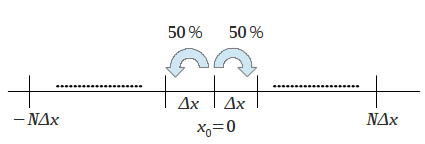
\includegraphics[scale=0.5]{figures/derive_diffusion_random_walk.png}
\end{center}
\caption{Deriving solution from Random-Walks \label{derive diffusion}}
\label{fig_step}
\end{figure}

Define $P(m,n)$ to be the probability that the particle
is at a point $m$ steps from $x_0$ after $n$ time steps. Then,
$x=m\delx$ and $t=n\delt$. Define $a$ and $b$ to be the number of
steps to the right and left, respectively. Then,

\begin{equation}
\begin{cases}
m=a-b\\
n=a+b
\end{cases}\Rightarrow\begin{cases}
a=\frac{m+m}{2}\\
b=\frac{n-m}{2}
\end{cases}.
\end{equation}

\indent Also, the number of possible paths from $x_0$ to the location $m\delx$ in
$n$ time steps is
\begin{equation}
    \frac{n!}{a!b!}=C^n_a.
\end{equation}
 Which is the binomial coefficient. 
 
The total number of possible paths to any position in the interval
[-$n\delx$, $n\delx$] is $2^n$. Thus, the probability we desire is
given by
\begin{equation}\label{P1}
    P(m,n)=\frac{\mbox{ \# of paths that reach m }}{\mbox{ total \# of possible paths }}=\frac{1}{2^n}\frac{n!}{a!b!}.
\end{equation}

\indent We would like to think of the continuous limit. If we consider
$\delx$ and $\delt$ to shrink to zero, $m$ and $n$ get large. We'll
therefore approximate the factorials in equation (\ref{P1}) by Stirling's Formula

\begin{equation}
    n!\sim(2\pi{}n)^{\frac{1}{2}}n^ne^{-n}, \text{where } n\gg 1.
\end{equation}

\noindent Our approximated probability is given by
\begin{equation}
    P(m,n)\sim \left(\frac{2}{n\pi}\right)^{\frac{1}{2}}\exp\left[\frac{-m^2}{2n}\right].
\end{equation}

\noindent Now we express this in terms of $x$ and $t$ to have

\begin{align}
P\left(\frac{x}{\triangle x},\frac{t}{\triangle t}\right) & \sim\left(\frac{2}{\frac{t}{\triangle t}\pi}\right)^{\frac{1}{2}}\exp\left(\frac{-\frac{x^{2}}{\triangle x^{2}}}{2\frac{t}{\triangle t}}\right)\\
 & =\left(\frac{2\triangle t}{\pi t}\right)^{\frac{1}{2}}\exp\left(\frac{-x^{2}}{2t}\frac{\triangle t}{\triangle x^{2}}\right).
\end{align}

\noindent Multiplying $\frac{1}{2\triangle x}$ on both sides (since we really want to know the probability of finding the particle within $2\Delta x$ units of x) gives
\begin{equation}
\frac{1}{2\triangle x}P\left(\frac{x}{\triangle x},\frac{t}{\triangle t}\right)\sim\left(\frac{1}{4\triangle x^{2}}\frac{2\triangle t}{\pi t}\right)^{\frac{1}{2}}\exp\left(\frac{-x^{2}}{2t}\frac{\triangle t}{\triangle x^{2}}\right).
\end{equation}

\noindent Letting $\delx, \delt \rightarrow 0$ such that
$\frac{\delx^2}{2\delt}\rightarrow D$, a finite, nonzero number, yields
\begin{equation}\label{fundamental soln}
    P(x,t)= \left(\frac{1}{4\pi{}Dt}\right)^{\frac{1}{2}}\exp\left[\frac{-x^2}{4Dt}\right].
\end{equation}

\noindent
It turns out that this is the fundamental solution to the 1-D diffusion
equation, meaning it solves the diffusion equation with Dirac Delta ``function" as an initial condition:
\begin{equation}
    \frac{\partial{}C}{\partial{}t}=DC_{xx}, \quad C(x,0)=\delta(x).
\end{equation}

This is circumstantial evidence that such random walk processes are
a mechanism underlying diffusion. If the properties of the random
walk are altered, for instance by biasing the walk in one direction,
different solutions will be obtained. This approach has been used in
attempts to derive models for chemotaxis, where other derivation
approaches become counterintuitive.

\subsection{Deriving PDE from Random Walks}
\indent
Consider a particle moving on a lattice that moves to the right with
probability $\alpha$ and to the left with probability $\beta$. The
particle moves by $\delx$ at each time step $\delt$, so the
probability of finding the particle at position $x_0$ is
\begin{equation}
    P(x,t)=\alpha{}P(x-\delx,t-\delt) + \beta{}P(x+\delx,t-\delt).
\end{equation}

We assume that $P(x,t)$ is smooth enough to allow the Taylor series
expansions of $P(x-\delx,t-\delt)$ and $P(x+\delx,t-\delt)$ about
the point $(x,t)$
\bea
    P(x-\delx,t-\delt)&\approx&P(x,t)-\delx{}P_x(x,t)-\delt{}P_t(x,t) +\nonumber \\
    && \frac{1}{2}[\delx^2P_{xx}(x,t)+2\delx\delt{}P_{xt}(x,t)+\delt^2P_{tt}(x,t)]\nonumber  \\
    P(x+\delx,t-\delt)&\approx&P(x,t)+\delx{}P_x(x,t)-\delt{}P_t(x,t) +\nonumber  \\
   & & \frac{1}{2}[\delx^2P_{xx}(x,t)-2\delx\delt{}P_{xt}(x,t)+\delt^2P_{tt}(x,t)]\nonumber
\ena

Assuming that $\alpha=\beta$ and $\alpha+\beta=1$, we obtain
\bea
    P(x,t)=P(x,t)-\delt P_t(x,t)+\frac{1}{2}\left[\delx^2P_{xx}(x,t)+\delt^2P_{tt}(x,t)\right],
\ena
or
\bea
    P_t(x,t)=\frac{\delx^2}{2\delt}P_{xx}(x,t)+\frac{\delt}{2}P_{tt}(x,t).
\ena

To move to the continuum description, we take the limit $\delx,
\delt  \rightarrow 0$ such that $\frac{\delx^2}{2\delt}  \rightarrow
D$, a finite number. This yields the diffusion equation,
\begin{equation}
    \frac{\partial{}P}{\partial{}t}=DP_{xx}.
\end{equation}

Again, if we modify the assumptions about $\alpha$ and $\beta$, we
can obtain different models, for example including advection effects.

\subsection{Derivation of general PDE by Conservation Law}
Our assumptions are that motion occurs in a homogeneous tube which we treat as a single space dimension and cross-sectional area is constant along its length.

Let $x$ be the distance along the tube from some arbitrary location. If we define $c$ to be the concentration/density of some particles, then we can ask what changes the density in some local neighborhoods $(x, x+\Delta x)$? Conservation implies that the only way to change the number (density) of particles is if a) particles move into or out of the region or b) particles are created or destroyed (born or die).

Let $c(x,t)$ be the concentration of particles(number of particles/volume). Let $J(x,t)$  be the flux of particles at location $x$ (number of particles crossing location $x$ at time $t$ (measure from left to right)). Let $\sigma(x,t)$ be the number of particles created or destroyed. Conservation implies

\begin{equation}
	\textrm{$\Delta$ concentration per time}=\text{rate of entry - rate of exit $\pm$ product/destruction}
\end{equation}

Let A be the cross-sectional area of tube and $\Delta V= A \Delta x$ . Then,
\begin{equation}
\frac{\partial}{\partial t} (c A \Delta x) = J(x,t)A-J(x+\Delta x ,t) A \pm \sigma(x,t)A \Delta x .
\end{equation}

A flux in the positive $x$ direction contribute to the net population positively at $x$, but negatively at $x+\Delta x$. Dividing by $A \Delta x$ is constant by assumption, we have

\begin{equation}
\frac{\partial c(x,t)}{\partial t}= \frac{J(x,t)-J(x+\Delta x,t)}{\Delta x} \pm \sigma(x,t).
\end{equation}
 Taking a limit as $\Delta x  \rightarrow 0$, we get the one dimensional balance equation

\begin{equation}
\frac{\partial c(x,t)}{\partial t}= \frac{-\partial J(x,t) }{\partial x} \pm \sigma(x,t).
\end{equation}

\noindent This is the general statement that can be applicable to several situations. Flux term J and $\sigma$ can be chosen differently.

  \begin{enumerate}
  \item Advection/Convection Equation: If particles are moving with a velocity $V$, then $J= k c V$ and substituting for a flux term gives $\frac{\partial c}{\partial t} = -\nabla (c k V)$ which is a closed dynamical system for c . When V is constant, it turns out 1D transport equation which is called advection/convection equation.

Net flux is  $J=c \alpha \nabla \psi $ where $\psi$ is given as some source of attraction of particles like nutrient signal or quorum sensing signal. If particles are charged, it can be electric potential also.

\item Diffusion Equation: For $J= -D \nabla c$ where D is the diffusion coefficient we can write the Fick's Law as
\begin{equation}
\frac{\partial c}{\partial t}= -\nabla \cdot(-D \nabla c)= D \nabla\cdot(\nabla c)= D \Delta c.
\end{equation}

\item  Diffusion+Advection Equation:  For the flux term $J=-D \nabla c +\alpha c V$, we have
\begin{equation}
\frac{\partial c}{\partial t}= -\nabla \cdot J= D \Delta c -\nabla (\alpha V c).
\end{equation}
\end{enumerate}

\subsection{Special Solution}
Consider the diffusion equation
\bea
   \frac{\partial c}{\partial t} = D \Delta c.
\ena
To make the problem well-posed, restrictions such as boundary conditions or initial conditions should be imposed.

\begin{enumerate}
\item{Infinite space domain with Dirac-Delta function} \\
The solution turns out to be the fundamental solution in \eqref{fundamental soln}.

\item{Finite space domain } \\
Let $\Gamma$ be the boundary. There are three types of boundary conditions:
	\begin{enumerate}
		\item{Dirichlet:} $c|_{\Gamma}=g$
		\item{Neumann:} $\frac{\partial c}{\partial t}|_{\Gamma}=g,\qquad \text{usually }g=0$
		\item{Robin:} $\alpha c|_{\Gamma}+\beta\frac{\partial c}{\partial t}|_{\Gamma}=g$
	\end{enumerate}
	Note that the Dirichlet boundary condition can always simplify to $c|_{\Gamma}=0$. Why? Suppose $c|_{\Gamma}=a$, then a rescaling $\tilde c=c-a$ satisfied the original diffusion equation and the boundary condition $\tilde c|_{\Gamma}=0$
	
\item{Time independent:}
\beq
	\frac{\partial c}{\partial t}=0\Rightarrow D\triangle c=0.
\eeq
The $c$ is the solution of the Laplace equation $D\triangle c=0$ and we call the solution $c$ is a steady-state solution.
\item{Spatially independent:} Solving
\beq
	\frac{\partial c}{\partial t}=0.
\eeq

\item{Traveling wave:} Discuss later.
\end{enumerate}

After making the PDE well-posed, a common trick to solve it is "Separation of variables". In our case, assume
\beq
	c(x,t)=X(x)T(t)
\eeq
where the form of $X$ and $T$ are determined by the boundary conditions. To find the solution of the diffusion equation, substitute $c(x,t)=X(x)T(t)$ into the diffusion equation and exploit the boundary/initial condition to find the answer of $c$.

When does separation of variables work? We use this ALL the time!
\subsection{Dimensional Analysis}
Consider the diffusion equation
\begin{equation}
  \frac{\partial c}{\partial t}= D \Delta c.
\end{equation}
A quick calculation using dimensional analysis can give us a crude estimate of diffusion coefficient $D$. Let fundamental parameters be length $L$, time $T$, and mass $M$. Then express every physical quantities into $L,t,M$. Denote the square bracket [ ] be the dimension of the physical quantity. So we have

\beq
	[c]=\frac{M}{L^{3}},\,[t]=T,\,[x]=L.
\eeq
Then

\begin{align}
\frac{\partial c}{\partial t}=D\frac{\partial^{2}c}{\partial x^{2}} & \Rightarrow\left[\frac{\partial c}{\partial t}\right]=\left[D\frac{\partial^{2}c}{\partial x^{2}}\right]\\
 & \Rightarrow\frac{M/L^{3}}{T}=[D]\frac{M/L^{3}}{L^{2}}\\
 & \Rightarrow[D]=\frac{L^{2}}{T}
\end{align}
The dimension to the diffusion coefficient $D$ is length square over time. By repeating experiment of
\[
\begin{cases}
\frac{\partial c}{\partial t}=DC_{xx}\\
c(0)=c_{0}\\
c(L)=0
\end{cases}
\]
and measuring how long does a particle (concentration) from $x=0$ to $x=L$. Since we have data for length and time, so the diffusion coefficient $[D]=L^{2}/T$ is obtained.

\noindent \textbf{Example}: Diffusion coefficient for 
$Oxygen (in air) \approx 10^{-1}$ $cm^2/s$. Estimate the time it takes for oxygen to equilibrate across a cell by diffusion? What about across a room?
(2) Smoke= $1.6 \times 10^{-2}$ $cm^2/s$ - it should be quite a bit smaller than oxygen since it is bigger\\

\noindent \textbf{Example}: In a 3m by 3m room diffusion of smoke from one corner to another corner, the time elapsed is
\begin{align*}
t & =\frac{L^{2}}{D}=\frac{(3\sqrt{2}*100)^{2}}{1.78*10^{-1}}\\
 & =1011235\,(s)\\
 & =280.89\,(hour)
\end{align*}

The elapsed time is far too long! Diffusion alone doesn't work. 
There are examples about bacterial sensing using diffusion.

%So it is not realistic and depends on the other conditions. Another possibility is a traveling wave solution to a reaction diffusion system.

\section{Traveling Wave Solutions}

\indent Reaction diffusion equation $u_t=Du_{xx}$ plus boundary conditions can be solvable with computers or analytically. We can talk about the perturbation/asymptotic solutions that we are interested.

Traveling wave is a  wave which travels without change of shape. If $u(x,t)$ is a travelling wave solution, the shape of the solution will be the same all time and the speed of propagation c will be a constant. Mathematically, we define as

\beq
	u(x,t)= u(x-ct)=u(z), \ z=x-ct.
\eeq
\noindent Then $u(x,t)$ is a travelling wave and it moves at constant speed c in the positive x direction. When we look for traveling wave solutions, we have

\begin{equation}
\frac{\partial u}{\partial t} = \frac{\partial u}{\partial z} \frac{\partial z}{\partial t}= -c \frac{du}{dz} \nonumber
\end{equation}
\begin{equation}
\frac{\partial u}{\partial x} = \frac{\partial u}{\partial z} \frac{\partial z}{\partial x}= \frac{du}{dz} \nonumber
\end{equation}
\begin{equation}
\frac{\partial^2 u}{\partial x^2} = \frac{d^2}{d z^2}.  \nonumber
\end{equation}

\noindent So, we have an ODE in traveling wave coordinates:
\begin{equation}
    Du''+cu'=0
\end{equation}
This is an eigenvalue problem for the wave speed $c$ and the wave
front profile function $u$. The solution is
\begin{equation}
    u=A+Be^{\frac{-cz}{D}}.
\end{equation}

On the infinite domain, since the exponential becomes unbounded as
$z \rightarrow-\infty$, so $B$ must be zero. Thus, $u=A$ and the
solution is a constant function and to be considered as a traveling wave.

\section{Fisher Equation}
The simplest case of a nonlinear reaction diffusion equation is
\begin{equation}
	u_t=u_{xx}+u(1-u)
\end{equation}

It was suggested by Fisher (1937) as a deterministic version of a stochastic model for the spatial spread of a favoured gene in a population. It is also the natural extension of the logistic growth population model.

In the spatially homogeneous situation the steady states are $u = 0$ and $u = 1$, which
are respectively unstable and stable. This suggests that we should look for travelling
wave solutions for which $ 0\leq u \leq 1$; negative $u$ has no physical meaning for such models.

Next, we look for traveling wave solutions. When we change to the traveling wave coordinate, we end up with the ODE:

\begin{equation}
    u''+cu'+u(1-u)=0
\end{equation}

Again, we'll require that the solution to this ODE is bounded.
Phase plane analysis will allow us to find the solutions we seek. In
the phase plane, trajectories that are bounded represent the profile
of a wave front. Steady states in the phase plane will be constant
solutions, and so are not interesting. We'll look for trajectories
such as heteroclinic and homoclinic orbits, and limit cycles.

We write our second order ODE as a system of first order ODEs:
\begin{align}
    u'&=w\\
    w'&=-cw-u(1-u)
\end{align}
This system has steady states at (0,0) and (1,0), and it's Jacobian
matrix is:
\begin{equation*}
\begin{pmatrix}
  0 & 1 \\
  -1+2u & -c \\
\end{pmatrix}
\end{equation*}

At (1,0), we have a saddle for all values of c. The eigenvalues are

\begin{center} $\lambda_{\pm}=-c/2\pm{}\sqrt{c^2+4}/2$. \\\end{center}

At (0,0), we have a stable node if $c^2 >4$ and stable spiral if $c^2 < 4$ with eigenvalues

\begin{center} $\lambda_{\pm}=-c/2\pm{}\sqrt{c^2-4}/2$.\\\end{center}

If $c<2$ there is a traveling wave solution but without biological meaning since $u<0$.
If $c>2$ there are traveling wave solutions.

$c=2$ is the most stable wave speed.

\begin{figure}[tbh]
\begin{centering}
\subfloat{\begin{centering}
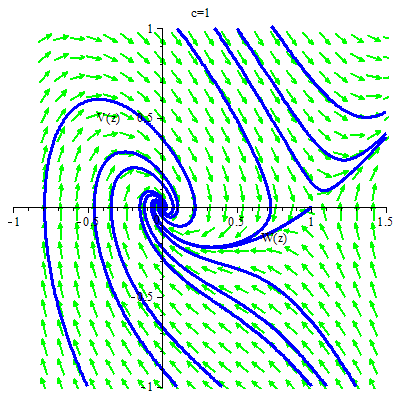
\includegraphics[width=5.4cm]{figures/solution_of_Fisher_equation_c=1}
\par\end{centering} }
\subfloat{\begin{centering}
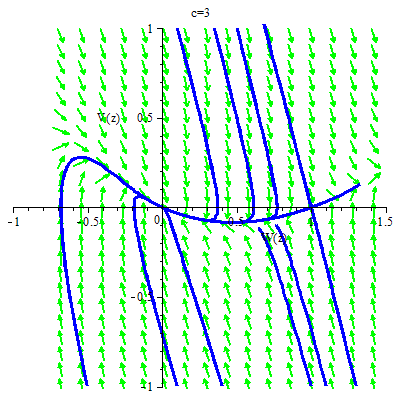
\includegraphics[width=5.4cm]{figures/solution_of_Fisher_equation_c=3.png}
\par\end{centering} }
\par\end{centering}
\caption{\label{figure:PF}Phase plane of solutions of Fisher's equation with different values of c}
\end{figure}


\section{Bistable(Cubic) Reaction Term}
Remembering FHN:

\bea
 \dt{v} &=& f(v)-w-w_0 \nonumber \\
\dt{w} &=& \epsilon(v-\gamma w-v_0)\nonumber
\ena
\noindent where $f(v) = Av(v-\alpha)(1-v)$ ($0<\alpha<1$). If the recovery variable ($w$) is fixed and we allow things to diffuse, we get something of the form:

\begin{equation}
u_t=u_{xx}+mu(u - 1)(\alpha - u), \ \ \ 0<\alpha<1
\end{equation}

Bistable equation and as a dynamics it looks like Fitz-Hugh Nagumo with diffusion and it is also a version of Cable Equation.
\newline
\noindent Are there travelling wave solutions? To check we apply the
change of variables.

\begin{equation}
u(x,t)=v(x+ct)=v(\xi) \nonumber
\end{equation}

\begin{equation}
cv_\xi =v_{\xi\xi} + m v(v-1)(\alpha-v) \nonumber
\end{equation}

\noindent For $f(v)=m v(v-1)(\alpha-v)$

\begin{center}
$v_{\xi}=w$

$w_{\xi}=cw-f(v)$\\
\end{center}

\noindent The steady states of f(v) are $v=0,1,$\,and\,$\alpha$. Now we are going to compute the Jacobian.


\begin{center}
$J(v,w)=
\begin{pmatrix}
  0 & 1 \\
  -f^{'}(v) & c \\
\end{pmatrix}$
\par\end{center}

Note that $-f^{'}(v)=-2mv\alpha+3mv^{2}+m\alpha-2mv$.
\newline\indent The Jacobians are

\begin{center}
$J(0,0)=
\begin{pmatrix}
  0 & 1 \\
  m\alpha & c \\
\end{pmatrix}$
\par\end{center}

$det(J(0,0))=-m$ $\alpha < 0$ \ \ $ \Rightarrow$ \ \ (0,0) is a saddle.

\begin{center}
$J(1,0)=
\begin{pmatrix}
  0 & 1 \\
  -m(\alpha-1) & c \\
\end{pmatrix}$
\par\end{center}

$det(J(1,0)) < 0$ \ \ $ \Rightarrow$ \ \ (1,0) is a saddle.


\begin{center}
$J(\alpha,0)=
\begin{pmatrix}
  0 & 1 \\
  -m\alpha(1-\alpha) & c \\
\end{pmatrix}$
\par\end{center}

$det(J(\alpha,0))=m\alpha(\alpha-1) > 0$ node or spiral depends on $\alpha$.

Stability depends on c. If c $>$ 0 it is unstable.


To determine the sign of c

\begin{equation}
\int_{-\infty}^{\infty} v_\xi(v_{\xi\xi}-cv_\xi+f(v)=0)d\xi \nonumber
\end{equation}

\begin{equation}
\int_{-\infty}^{\infty} \frac{d}{d\xi}(\frac{(v_\xi)^2}{2})d\xi-c\int_{-\infty}^{\infty}(v_\xi)^{2}d\xi+\int_{-\infty}^{\infty} f(v)v_\xi d\xi=0 \nonumber
\end{equation}


By a change of variables $s=u$


\begin{equation}
\int_{-\infty}^{\infty}\frac{d}{dz}(\frac{(u_\xi)^{2}}{2})d\xi-c\int_{-\infty}^{\infty}(u_\xi)^{2}d\xi+\int_{0}^{1}f(s)ds=0 \nonumber
\end{equation}


\indent Note: $\frac{(u_\xi)^{2}}{2}$ $\downharpoonright_{-\infty}^{\infty}=0$ if you move from FP to FP.


\begin{equation}
c=\unit{\frac{\int_{0}^{1}f(s)ds}{\int_{-\infty}^{\infty}(u_\xi)^{2}d\xi}} \nonumber
\end{equation}


Suppose $\int_0^1 f(s) ds > 0$ \ \ $ \Rightarrow$ c is positive.

Look for $c\approx0$ is the trajectory goes from $(0,0)$ to $(1,0)$.

\begin{equation}
\int_{-\infty}^{\infty} u_\xi(u_\xi+f(u)=0)d\xi \nonumber
\end{equation}
\begin{equation}
\int_{-\infty}^{\infty} \frac{d}{d\xi}(\frac{u_\xi^2}{2})d\xi+\int_0^1 f(s)ds \nonumber
\end{equation}
\begin{figure}
\caption{Notes for bistable}
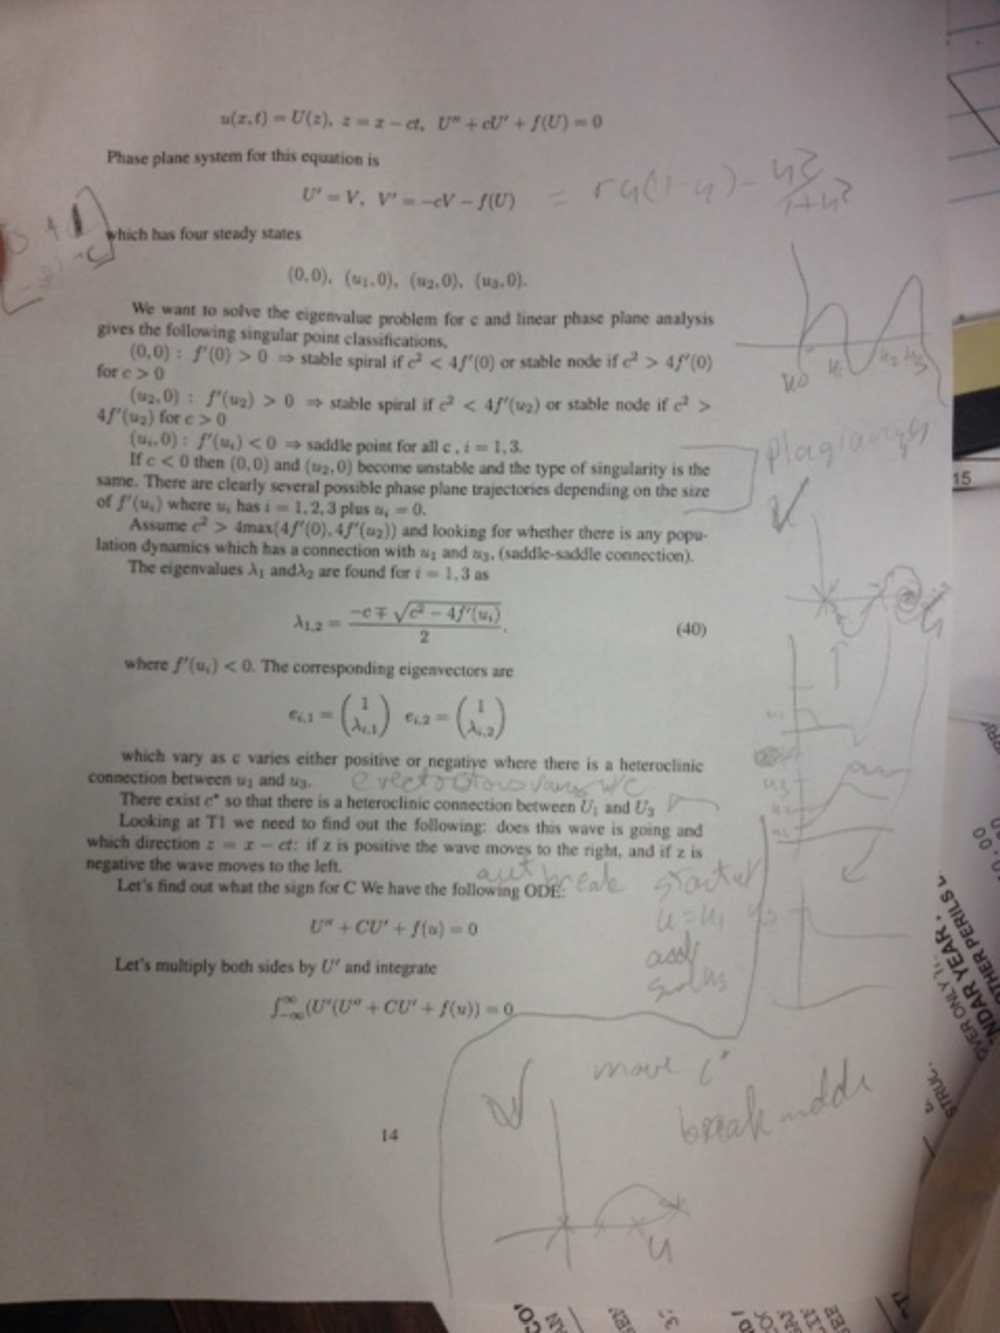
\includegraphics[scale=.65]{figures/bistable.pdf}
\label{fig_bist}
\end{figure}

Since the terms are all positive , there is no traveling wave when $c=0$.

Summary: $u_t=u_{xx}+f(u)$

{\bf 1)} If $f(u)=0$, no traveling waves.

{\bf 2)} If  $f(u)=u(1-u)$, traveling waves with numerous speeds.

{\bf 3)} If $f(u)=$ cubic, one traveling wave for specific c.

{\bf 4)} If $f(u)=$ higher order, a practical example of growth function for spruce budworm problem.


\subsection{Spruce-Budworm Problem}
This is an ODE model as

\begin{equation}
\frac{du}{dt}=f(u)
\end{equation}
with
\begin{equation}
f(u)=ru(1-u)-\frac{u^2}{1+u^2}
\end{equation}

Analyze this here!
SS:

Solve 
\bea
0 &=& f(u) \nonumber \\
&=& ru(1-u)-\frac{u^2}{1+u^2} \nonumber
\ena
$u=0$ is one solution. The other satisfies $r(1-u)-\frac{u}{1+u^2}=0$
plot this as the linear part and nonlinear part intersecting and see that there are up to 3 additional eq. When there are three you have:

$0 ---->u_1<----u_2----->u_3<-----$ implying $u_1$ is stable and referred to as a refuge population. add too many and tend to $u_3$, the outbreak case. Consider spatial aspects.

\noindent Let us look for travelling wave solutions

\begin{center}
$u(x, t) = U(z)$,\ \ $ z = x - ct $, \ \ $ U''+cU'+ f (U) = 0$\\
\end{center}

\noindent Phase plane system for this equation is

\begin{center}
$U'= V$,\ \ \ $ V'=-cV - f (U)$ \\
\end{center}

\noindent which has four steady states

\begin{center}
$(0, 0),\ \  (u_1, 0),\ \  (u_2, 0),\ \  (u_3, 0)$.\\
\end{center}

We want to solve the eigenvalue problem for c and linear phase plane analysis gives the following singular point classifications,

$(0,0):$ \ $ f'(0)> 0 $ \ $ \Rightarrow$ stable spiral if $c^2<4 f'(0)$ or stable node if $c^2> 4f'(0)$ for $c>0$

$(u_2,0):$ \ $ f'(u_2)> 0 $ \ $ \Rightarrow$ stable spiral if $c^2<4 f'(u_2)$ or stable node if $c^2> 4f'(u_2)$ for $c>0$

$(u_i,0):$ \ $ f'(u_i)< 0 $ \ $ \Rightarrow$ saddle point for all c , $i=1,3$.

If $c < 0$ then $(0, 0)$ and $(u_2, 0)$ become unstable and the type of singularity is the same.
There are clearly several possible phase plane trajectories depending on the size of $f'(u_i )$ where $u_i$ has $i = 1, 2, 3$ plus $u_i = 0.$

Assume $c^2 > 4 $max$ (4f'(0),4f'(u_2))$ and looking for whether there is any population dynamics which has a connection with $u_1$ and $u_3$, (saddle-saddle connection).

The eigenvalues $\lambda_1$ and$\lambda_2$ are found for $i=1,3$ as
\begin{equation}
\lambda_{1,2} = \frac{-c \mp \sqrt{c^2-4f'(u_i)} }{2}.
\end{equation}

where $f'(u_i)<0$. The corresponding eigenvectors are
\begin{center}
$e_{i,1}= \begin{pmatrix} 1 \\ \lambda_{i,1} \end{pmatrix} $ \ \ $e_{i,2}= \begin{pmatrix} 1 \\ \lambda_{i,2} \end{pmatrix} $
\end{center}

which vary as c varies either positive or negative where there is a heteroclinic connection between $u_1$ and $u_3$.

There exist $c^*$ so that there is a heteroclinic connection between $U_1$ and $U_3$

Looking at T1 we need to find out the following: does this wave is going and which direction $z = x - ct$: if z is positive the wave moves to the right, and if z is negative the wave moves to the left.

Let's find out what the sign for C
We have the following ODE:

\begin{center}
$U'' + CU' + f(u) = 0$
\end{center}

Let's multiply both sides by $U'$ and integrate

\begin{center}
$\int _{-\infty}^{\infty} (U' (U''+CU'+f (u ) )=0$
\end{center}

\begin{align}
\int_{-\infty}^{\infty}\frac{1}{2}\frac{d({U}')^2}{dz}dz+\int_{-\infty}^{\infty}C(U^{'})^{2}dz+\int_{-\infty}^{\infty}f(U)U^{'}dz & =0\\
\frac{U^{'}}{2}|_{-\infty}^{\infty}\nonumber+C\int_{-\infty}^{\infty}(U^{'})^{2}dz\nonumber+\int_{U_{3}}^{U_{1}}f(S)ds=0
\end{align}

\begin{align}
C\int_{-\infty}^{\infty}(U^{'})^{2}dz\nonumber=-\int_{U_{3}}^{U_{1}}f(S)ds
\end{align}

The sign of $C = -sign (\int _{U_3}^{U_1}f (S )ds )$

\subsection{Growth of Cell Cluster}
Some biologist sometimes need to grow tissue (or biofilm) they dropped pieces of bacteria in a beaker. Below are some assumptions about the processes.

\begin{itemize}
	\item All clusters of bacteria are spheres.
	\item All clusters have the same initial size.
	\item Growth (rate of change of volume) of the clusters is related to surface area.
\end{itemize}
\begin{center}
$\dfrac{dv}{dt}=ks$
\end{center}
\begin{center}
$V=\frac{4}{3}\pi r^{3}$
\end{center}
\begin{center}
$S=4\pi r^{2}$
\end{center}

Where $v$ is the volume, $s$ is the surface area, and $r$ is the radius of each cluster. Taking the derivative of $v$ with respect to $r$ we get:
\begin{center}
$\dfrac{dv}{dt}=4\pi r^{2}\frac{dr}{dt}=k4\pi r^{2}$ 
\end{center}
dividing both sides by $4\pi r^{2}$ yields:
\begin{center}
$\dfrac{dr}{dt}= k$
\end{center}
\begin{center}
$V_{0}= v_{0}*N $
\end{center}


Where $V$ is the total volume and $N$ is the number of spheres. Solving for $r$ gives:


\begin{center}
$r = kt+r_{0}$
\end{center}

Thus the total volume is given by:

\begin{center}
$V = N\frac{4}{3}\pi(kt+r_{0})$ 
\end{center}

\begin{itemize}
\item Now we will assume the clusters no longer have the same initial size.
\end{itemize}

The spheres have initial distribution $\alpha(r)$. Assume each sphere grows like:
\begin{center}
 $\dfrac{dr}{dt}=k$.
 \end{center}

Let $p(r,t)$ be the number of sphere of radius $r$ at time $t$. The following integral determines the proportion of clusters with radius between $[r,r + \Delta r]$ at time $t$.
\begin{center}
$\int_{r}^{r+\Delta}p (r,t )dr$
\end{center}




We set Boundary conditions of $P(\infty, t )=0$ and $P (0,t )=0$. We use the following equation to determine $p$.

\begin{center}
$p_{t} = -kp_{r}$
\end{center} 

We will not motivate this rigorously, or even at all. Just think as about and try to convince yourself it makes sense. This is a common PDE that we know has traveling wave solutions. We look for these solutions by doing the following:

\begin{center}
$P (r,0 )=\alpha (r )$, $P (0,t )= 0$
\end{center}
\begin{center}
$Z = r - ct$  (traveling wave)
\end{center}
\begin{center}
$P (r,t )= P (r-ct )$
\end{center}
\begin{center}
$-cP_{z}=-kP_{z}$
\end{center}

For this ODE the have a solution, $c=k$. So we know that the total volume is given by the following integral:

\begin{center}
$V(t) = \frac{4}{3}\pi \int_{0}^{\infty} r^{3}p(r-kt)dr $
\end{center}
By substituting $u= r-kt$ we get:

\begin{center}
$V(t) = \frac{4}{3}\pi \int_{0}^{\infty}(u+kt)^{3}p(u)du $
\end{center}

\begin{center}
 $= \frac{4}{3}\pi \int_{0}^{\infty}(u+kt)^{3}p(u)du $
\end{center}

\begin{center}
$ = [V_{0} + ktS_{0}+4\pi(kt)^{2}R_{0}+4/3(kt)^{3}] N_{0}$
\end{center}

\begin{center}
$N(t) = \int_{0}^{\infty}p(r,t)dr$
\end{center}

\noindent First Moment-Radius:
$R = \frac{1}{N (t )}\int _{0}^{\infty} rP (r,t )dr$

\noindent Second Moment-Surface Area:
$S (t )=\frac{4\pi}{N}\int _{0}^{\infty} r^{2}P (r,t )dr$

\noindent Third Moment-Volume:
$V = \frac{4\pi}{3}\frac{1}{N}\int _{0}^{\infty} r^{3}P (r,t )dr$

\subsection{Chemotaxis}
Here we have 2 constituents:
\begin{itemize}
	\item Bacteria, which consume nutrient and grow. Bacteria have random and directed motion which is signal/nutrient dependant.
	\item Signal/nutrient, which is consumed and diffuses.
\end{itemize}

Here we denote $b(x,t)$ as bacteria and $s(x,t)$ as signal.
\begin{center}
$\dfrac{\partial b}{\partial t} + (J)_{x}=f(s,b)$
\end{center}
\begin{center}
$J=J_{diffusion}+J_{chemotaxis}$
\end{center}
\begin{center}
$\dfrac{\partial b}{\partial t}=f(s,b)+(Db_{x})_{x}-(b\chi(s)s_{x})_{x}$
\end{center}

We will consider $D$ as a constant so $(Db_{x})_{x}=Db_{xx}$. $\chi(x)$ is how sensitive the bacteria is to the signal. Intuitively, the more nutrient available the less sensitive the bacteria should be to it. Possible expressions are $\chi(x) = \dfrac{\chi_{0}}{s}$ or $\chi(x)=\dfrac{\chi_{0}k}{(k+s)^{2}}$.

\begin{center}
$\dfrac{\partial s}{\partial t}=-g(s,b) + (D_{s}s_{x})_{x}$
\end{center}

We make two assumptions
\begin{itemize}
\item $f=0$
\item $D_{s}=0$
\end{itemize}

This yields the following equations:

\begin{center}
$\dfrac{\partial b}{\partial t}=\dfrac{\partial}{\partial x}(Db_{x}-b\chi(s)s_{x})$
\end{center}

\begin{center}
$\dfrac{\partial s}{\partial t}=-k(s)b$
\end{center}

\noindent Initial conditions are given by $b(x,0)=b_{0}$ and $s(x,0) = s_{0}$. We consider  $0<x<L$ with boundary conditions $\dfrac{\partial b}{\partial x} = \dfrac{\partial s}{\partial x} = 0$ at $x=0,L$. Now we look for traveling wave solutions. 

\begin{center}
$z=x-ct$
\end{center}

\bea
cb'&=&-Db''+b(\chi(s)s')'\nonumber \\
&=&-Db''+(\delta \frac{b}{s} s')' \nonumber
\ena
\begin{center}
$cs'=k(s)b$
\end{center}
We have BC that imply that $b\rightarrow 0$, $b'\rightarrow 0$, $s\rightarrow s_{\infty}$ as $z\rightarrow\infty$
Which is equivalent to assuming far in front of the wave front there are no bacteria and s is the initial value.
 Integrate first equation
\bea
cb=-Db'+\dfrac{bx_{0}s'}{s}+Q 
\ena

$Q$ is zero from boundary conditions.
\bea
b'&=&-\frac{c}{D}b+\dfrac{b\chi_{0}s'}{D_{s}} \nonumber \\
\frac{b'}{b} &=&-\frac{c}{D}+\dfrac{\chi_{0}s'}{D_{s}} \nonumber
\ena
Integrate and find that $b=\hat Q S^{\delta/D}e^{-z}$
Substitute into previous equation, integrate:

$$s=(Qkc^{-2}(\delta-D)e^{-cz/D}+s_0^{1-\delta/D})^{-\frac{1}{\delta/D-1}}$$ 
This system of ODEs has a closed form solution given by:

%\begin{center}
%$b(z)=\dfrac{c^{2}s_{0}}{k(\chi_{0}-D)}(\dfrac{s}{s_{0}})^{\frac{\chi_{0}}{D}}e^{-\frac{cz}{D}}$
%\end{center}
%
%\begin{center}
%$s(z)=s_{0}(1+e^{-\frac{cz}{D}})^{-\frac{D}{\chi_{0}-D}}$
%\end{center}
\section{Calcium Waves}
Calcium waves: calcium induce (CI) and calcium release (CR), molecular switch, ODE model CI CR dynamics
Small influx of calcium releases a large amount from some storage membrane within the cell (ER).
$u$ be the calcium concentration within the cytosol:
\bea
\underbrace{\frac{du}{dt}}&=& \underbrace{L}-\underbrace{ru}+\underbrace{A (u )} \\ \nonumber
\textrm{rate of change}  && \parbox{1cm}{\textrm{leak from ER}}  \parbox{1cm}{\textrm{uptake to ER}} \hspace{.2cm}   \parbox{1cm}{\textrm{Induced realease}  }
\ena

   $u$ is the concentration of external calcium there 3 things to look for: $L$ - leak, $ru$ - uptake by the membrane, and $A(u)$- release

   \begin{center}
   $\frac{du}{dt}= L + \frac{k_{1}u^{2}}{k_{2}+u^{2}}-k_{3}u$
   \end{center}
   if $L=0$ then there are three SS:
Sketch them here

Very complicated nonlineariity, so make it simpler:
\bea
 f(u)= A (u-u_{1} ) (u_{2}-u ) (u-u_{3} )
 \ena

   $u_{t}= f (u )+D\Delta u$


   Travelling wave solution: $u (x,t )= U (z )$ where $z = x-ct$ and $U(-\infty) = u_{3}$,  $ U(\infty) = u_{1}$

   \begin{center}
   $DU'' + CU'+ A (u-u_{1} ) (u_{2}-u ) (u-u_{3} )=0$
   \end{center}
Move on to phase=plane analysis or pull a murray....
   Now, try to find solution U that satisfies

   $$U' = A (u-u_{1} ) (u-u_{3} )\\$$

    $$l [u ]=(u-u_{1} ) (u-u_{3} ) \{ (2Da^{2}-A )- [Da^{2} (u_{1}+u_{3} )-ca-Au_{2} ] \}=0$$

    From this get $$2Da^{2}-A=0$$ and  $$Da^{2} (u_{1}+u_{3})-ca-Au_{2} =0$$

   $$a =  (\frac{A}{2D} )^{\frac{1}{2}}$$
   $$c=(\frac{A}{2D} )^{\frac{1}{2}}(u_{1}-2u_{2}+u_{3} )\\$$




\subsection{2D}
   In two dimensions, $U_{t}=f(u)+D\Delta u$ is the surface of  a sphere of radius R.

   \begin{center}
   		$U_{t} = f(u)+(\frac{1}{R^{2}} [u_{\theta\theta}+cot\theta\frac{du}{d\theta}]$
   \end{center}

   Local pulse of calcium

  $$ U (\theta,t )=U (z ),  z=R\theta-ct$$

  $$ DU''+ [c+\frac{D}{R}cot\theta ]U'+A (u-u_{1} ) (u_{2}-u ) (u-u_{3} )$$

   $$C =  (\frac{AD}{2} )^{\frac{1}{2}} (u_{1}-2u_{2}+u_{3} )-\frac{D}{R}cot\theta$$
	\[
\]

%%%%Jemison
\newpage
\section{Belousov-Zhabotinskii Reaction}
One of the differences that the BZ reaction has, relative to the previous set of examples is that it is not a scalar system. This requires several areas of attention.
The Belousov-Zhabotinskii reaction (BZ reaction) is an example of an oscillating reaction. Assuming a spatially homogeneous medium, a model for an oscillating reaction is of the form 
\begin{equation}\label{nonlin}
\frac{d}{dt} \vec{u} = f(\vec{u}),
\end{equation}
where $\vec{u}$ is the concentration vector and $f$ describes the reaction kinetics. The components of $\vec{u}$ are the concentrations of the chemicals involved in the reaction (Murray, VI, p.220). We will look for periodic solutions to (\ref{nonlin}) such that
\begin{equation}
\vec{u}(t+T)=\vec{u}(t)
\end{equation}
where $T>0$ is the period of the oscillation.
\subsection{Field-K\"{o}r\"{o}s-Noyes (FKN) Model}
Many chemical reactions come into play to produce the BZ reaction. The Field-K\"{o}r\"{o}s-Noyes or FKN model involves 5 key reactions which capture the basic oscillatory mechanism observed in the BZ reaction. These five reactions can be represented by a system involving 3 chemicals (Murray, Volume I, p.259).
 

The chemical elements involved in the 5-reaction FKN model are as follows:

\begin{center}
$\begin{array}{l l}
X = & H Br O_2 \\
Y = & Br^- \\
Z = & Ce^{4+} \\
A = & BrO_3^- \\
P = & HOBr
\end{array} $
\end{center}


This gives us the following stoichiometry where $f \sim 0.5$ is a stoichiometric factor, and $k_{1} \ldots k_{5}$ are rate constants.

\begin{center}
$\begin{array}{l c l}
A + Y & \xrightarrow{\text{k1}} & X + P \\
X + Y & \xrightarrow{\text{k2}} & 2P \\
A + X & \xrightarrow{\text{k3}} & 2X + 2Z \\
2X & \xrightarrow{\text{k4}} & A + P \\
Z & \xrightarrow{\text{k5}}& fY
\end{array} $
\end{center}

Using the Law of Mass Action to turn the above into differential equations, we obtain the following third-order system where lowercase letters are used for the chemical concentrations, i.e, [$X$] $=x$, [$Y$] $=y$, etc. (Murray, Volume I, p.260)  
\bea
\label{sys_1}
\cfrac{dx}{dt} & = & k_1 ay - k_2 xy + k_3 ax - k_4 x^2\\
\label{sys_2}
\cfrac{dy}{dt} & = & -k_1 ay - k_2 xy + f k_5 z \\
\label{sys_3}
\cfrac{dz}{dt} & = & 2k_3 ax - k_5 z
\ena
Re-scaling and nondimensionalising (\ref{sys_1})-(\ref{sys_3}), we get

\bea
\label{e_dx}
\epsilon \cfrac{dx}{dt} & = & qy - xy + x(1-x) \\
\label{d_dy}
\delta \cfrac{dy}{dt} & = & -qy - xy + 2f z \\
\label{1_dz}
\cfrac{dz}{dt} & = & x - z
\ena


\indent The system has three steady states, 2 stable and 1 unstable. ***put the details in here***The goal is to show that a limit cycle solution exists. Since the Poincar\'{e}-Bendixson theorem can only be applied in two dimensions, and we have a three-dimensional system, we need to take an approach where we can re-scale to show that the local behavior of the 3-D system around the unstable steady state approaches planar behavior. Then, we will be able to apply the Poincar\'{e}-Bendixson theorem to the 2-D approximation.

\indent We now assume that $x$ is not changing much, so $\frac{dx}{dt}$ is slow compared to $\frac{dy}{dt}$ and $\frac{dz}{dt}$. Based on that we set $\varepsilon=0$ in (\ref{e_dx}), which gives

$$0= -qy + xy - x(1-x)$$

Solving for $x$ as a function of $y$, we obtain
$$x(y)_{+}=\frac{1-y}{2}+\frac{\sqrt{(y-1)^2+4qy}}{2}$$
$$x(y)_{-}=\frac{1-y}{2}-\frac{\sqrt{(y-1)^2+4qy}}{2}$$
Since $x$ is concentration, it cannot be negative. Therefore, we can discard $x(y)_{-}$.
So, for the reduced system, we have
\bea
\label{d_dy1}
\delta \cfrac{dy}{dt} & = & -y[x(y)+q]+ 2f z \\
\label{1_dz1}
\cfrac{dz}{dt} & = & x(y) - z
\ena

From here, we have two choices for how to proceed. We could make an argument to set $\delta=0$ in (\ref{d_dy1}), solve for $y$ as a funcrion of $z$, and plug that in the $\frac{dz}{dt}$ equation. This reduction will result in a single ODE, which should be simple to analyze. However, by setting $\delta=0$, we lose even more information.

Another way, which will allow us to preserve information, is to to analyze the full system (\ref{d_dy1})-(\ref{1_dz1}). To obtain some intuition about how the system behaves, we can start by using pplane (Matlab). Using pplane, by trial and error, we see that in order to achieve a limit cycle, we need to select values for $q$ and $f$ in the following ranges:
$$q<1\hspace{1in}\frac{1}{4}<f<\frac{1+\sqrt{2}}{2}$$

These ranges can be derived analytically by finding the steady states of system (\ref{d_dy1})-(\ref{1_dz1}). Setting $\frac{dz}{dt}=0$, we get $x(y)=z$. We now need to plug $x(y)$ in 
$$-y[x(y)+q]+ 2f z=0$$
and solve for $y$. Finally, we need to find values for or $q$ and $f$ that make the steady state unstable. After this is achieved, we will be at the starting point in the application of the Poincar\'{e}-Bendixson theorem.

\begin{figure}
\caption{Trajectories in the phase plane for the reduced FKN model}
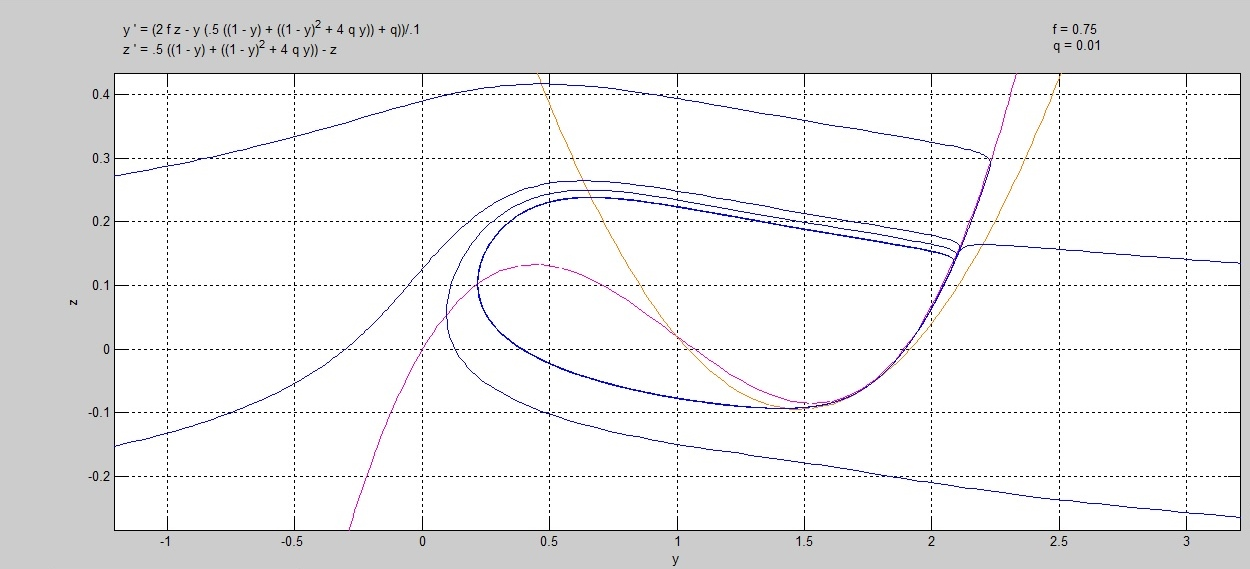
\includegraphics[scale=.45]{figures/FKN_figure.jpg}
\label{fig:fkn}
\end{figure}
Figure~\ref{fig:fkn} is a plot from pplane showing the $y$-nullcline (pink) and the $z$-nullcline(yellow) together with the course of some trajectories (blue), and we see that a limit cycle is starting to form. The final question to ask is: How can we interpret the solution to the system in (\ref{d_dy1})-(\ref{1_dz1}) in the context of the BZ reaction?

\section{Simplified Relaxation Oscillator}
A general model for a relaxation oscillator is given by
\begin{equation}\label{rox}
\varepsilon\frac{dx}{dt}=y-f(x)
\end{equation}
\begin{equation}\label{roy}
\frac{dy}{dt}=-x
\end{equation}
where $0<\varepsilon\ll 1$. Behavior of the system is governed by $f(x)$. In particular, we consider the van der Pol Oscillator, for which $f(x)=\frac{x^3}{3}-x$.
\newpage
\begin{equation}\label{fdpx}
\varepsilon\frac{dx}{dt}=y-\left( \frac{x^3}{3}-x\right) 
\end{equation}
\begin{equation}\label{fdpy}
\frac{dy}{dt}=-x
\end{equation}
Since $0<\varepsilon\ll 1$, $x$ changes fast compared to $y$. Figure~\ref{fig:vdp} shows how a trajectory moves in the phase plane, and Figure~\ref{fig:oscper} shows a plot of $x$ against $t$. 

We assume $\left( \varepsilon\frac{dx}{dt}\right) \ll 1$, and since $x$ changes fast, we can set $\varepsilon=0$. So, system (\ref{fdpx})-(\ref{fdpy}) becomes
\begin{equation}\label{fdpx1}
0=y-\left( \frac{x^3}{3}-x\right) 
\end{equation}
\begin{equation}\label{fdpy1}
\frac{dy}{dt}=-x
\end{equation}
This allows us to estimate the period ($T$) of the oscillation. 
Taking the derivative of (\ref{fdpx1}) with respect to $t$ and rewriting, we get
$$(x^2-1)\frac{dx}{dt}=\frac{dy}{dt}$$
$$(x^2-1)\frac{dx}{dt}=-x$$
$$\frac{x^2-1}{x}dx=-dt$$
We now integrate both sides. 
\begin{equation}\label{perT}
\int_2^{1} \frac{x^2-1}{x} \,dx = -\int_0^{\frac{T}{2}}\,dt 
\end{equation}
We would like to find half of the period, so the limits of integration for $t$ are 0 and $\frac{T}{2}$. In half the period we traverse the right branch of the cubic nullcline shown in Figure~\ref{fig:vdp}. The limits of integration for $x$ are obtained as follows:
\begin{itemize}
\item Set $f'(x)=\frac{x^2-1}{x}=0$ and solve for $x$. This gives $x=\pm1$,
\item Evaluate $f(-1)$. This gives $f(-1)=\frac{2}{3}$, 
\item Find the positive value for $x$ such that $f(x)=\frac{2}{3}$. This gives $x=2$.
\end{itemize}

Integrating (\ref{perT}) and solving for $T$ yields $T=3-2\ln 2$ for the estimate of the period.

It is not as simple to apply the method described above in the context of the FKN model for the BZ reaction because there is no symmetry between the right and the left branches of the cubic nullcline, as it is in the case of the van der Pol Oscillator. Also, the period for the FKN model changes with the value for the stoichiometric factor, $f$.

\begin{figure}
\caption{Phase plane for the van der Pol oscillator}
\begin{center}
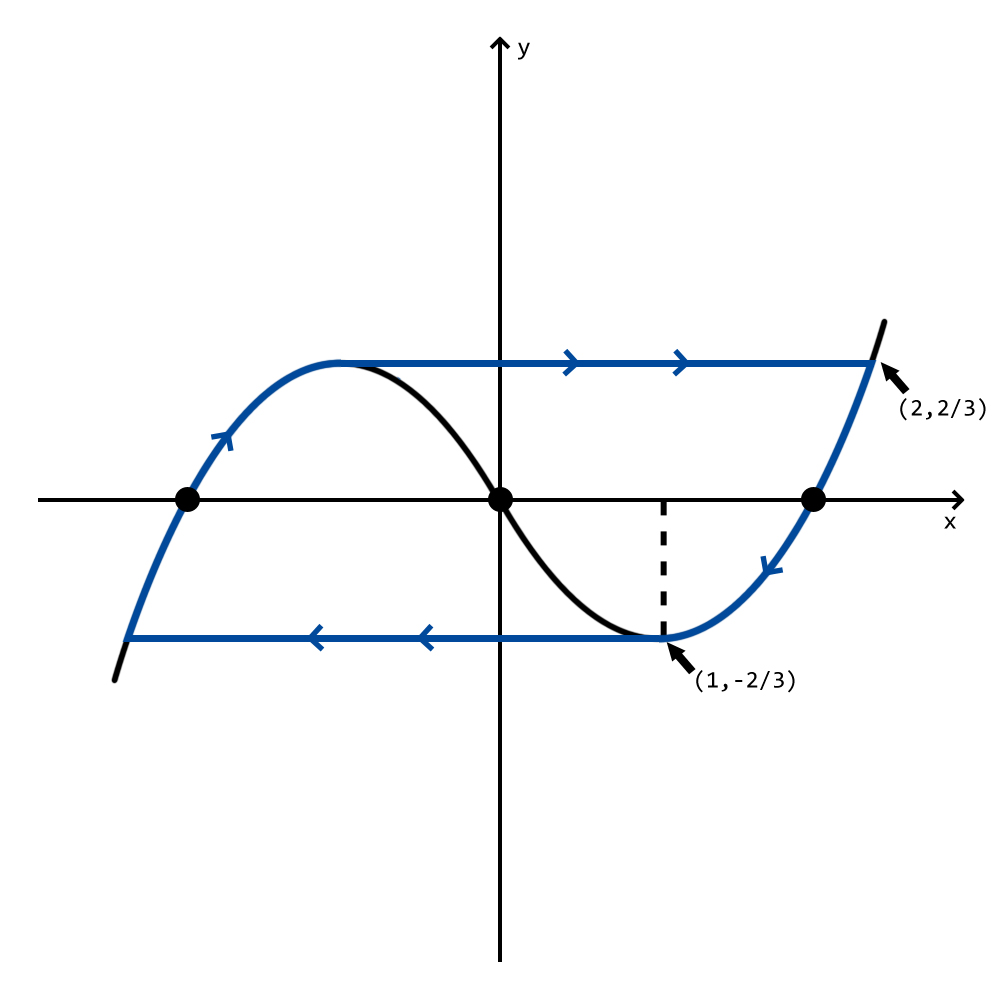
\includegraphics[scale=.25]{figures/van_der_Pol_oscillator.jpg}
\end{center}
\label{fig:vdp}
\end{figure}

\begin{figure}
\caption{Oscillations of $x$ in time}
\begin{center}
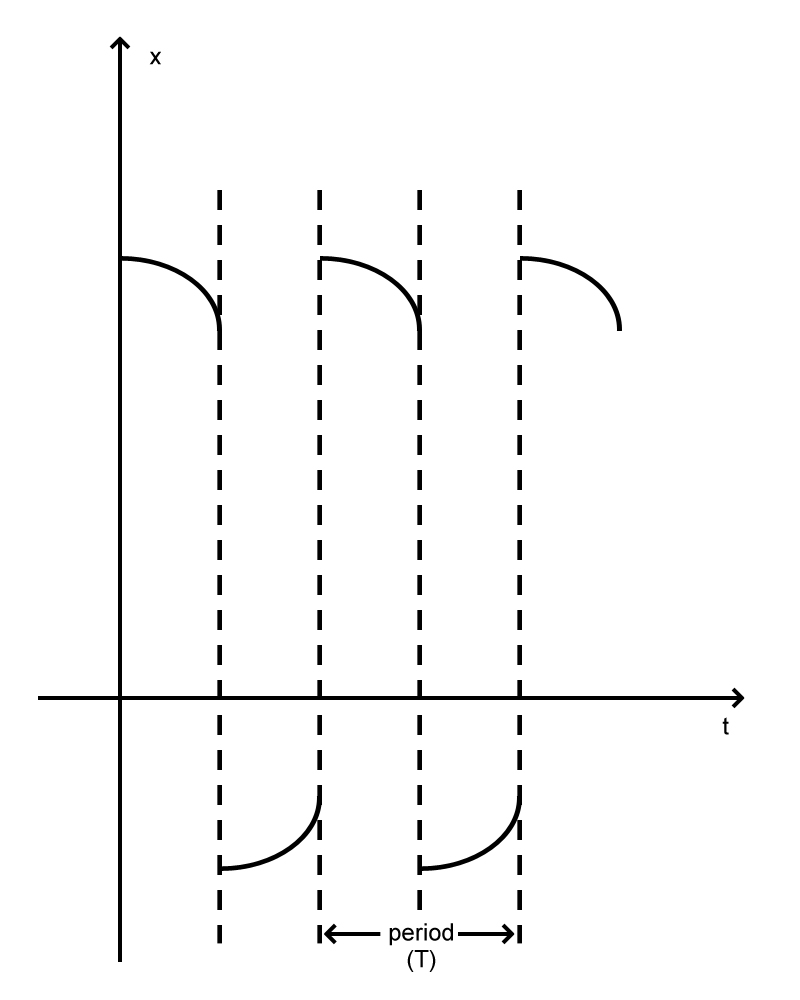
\includegraphics[scale=.20]{figures/Oscillator_period.jpg}
\end{center}
\label{fig:oscper}
\end{figure}

{\bf{Estimate the period for the BZ}}

We found earlier that $$x(y)_{+}=\frac{1-y}{2}+\frac{\sqrt{(y-1)^2+4qy}}{2}$$
and to get an estimate of the period, we will make the assumption that $q<<1$ and look at the nullclines from:

\bea
\label{d_dy1}
\delta \cfrac{dy}{dt} & = & -y[x(y)+q]+ 2f z \\
\label{1_dz1}
\cfrac{dz}{dt} & = & x(y) - z.
\ena

the $z$- nullcline is $ z=x(y) \approx 1-y$ if $q<<10y\leq 1$ and something else otherwise (I do not understand page 271 in Murray). The $y$ nullcline is $z=\frac{y(x(y)+q)}{2f}$. Depending on $f$ we can have three different regimes:
\begin{figure}[b!]
\caption{Null-clines}
\begin{center}
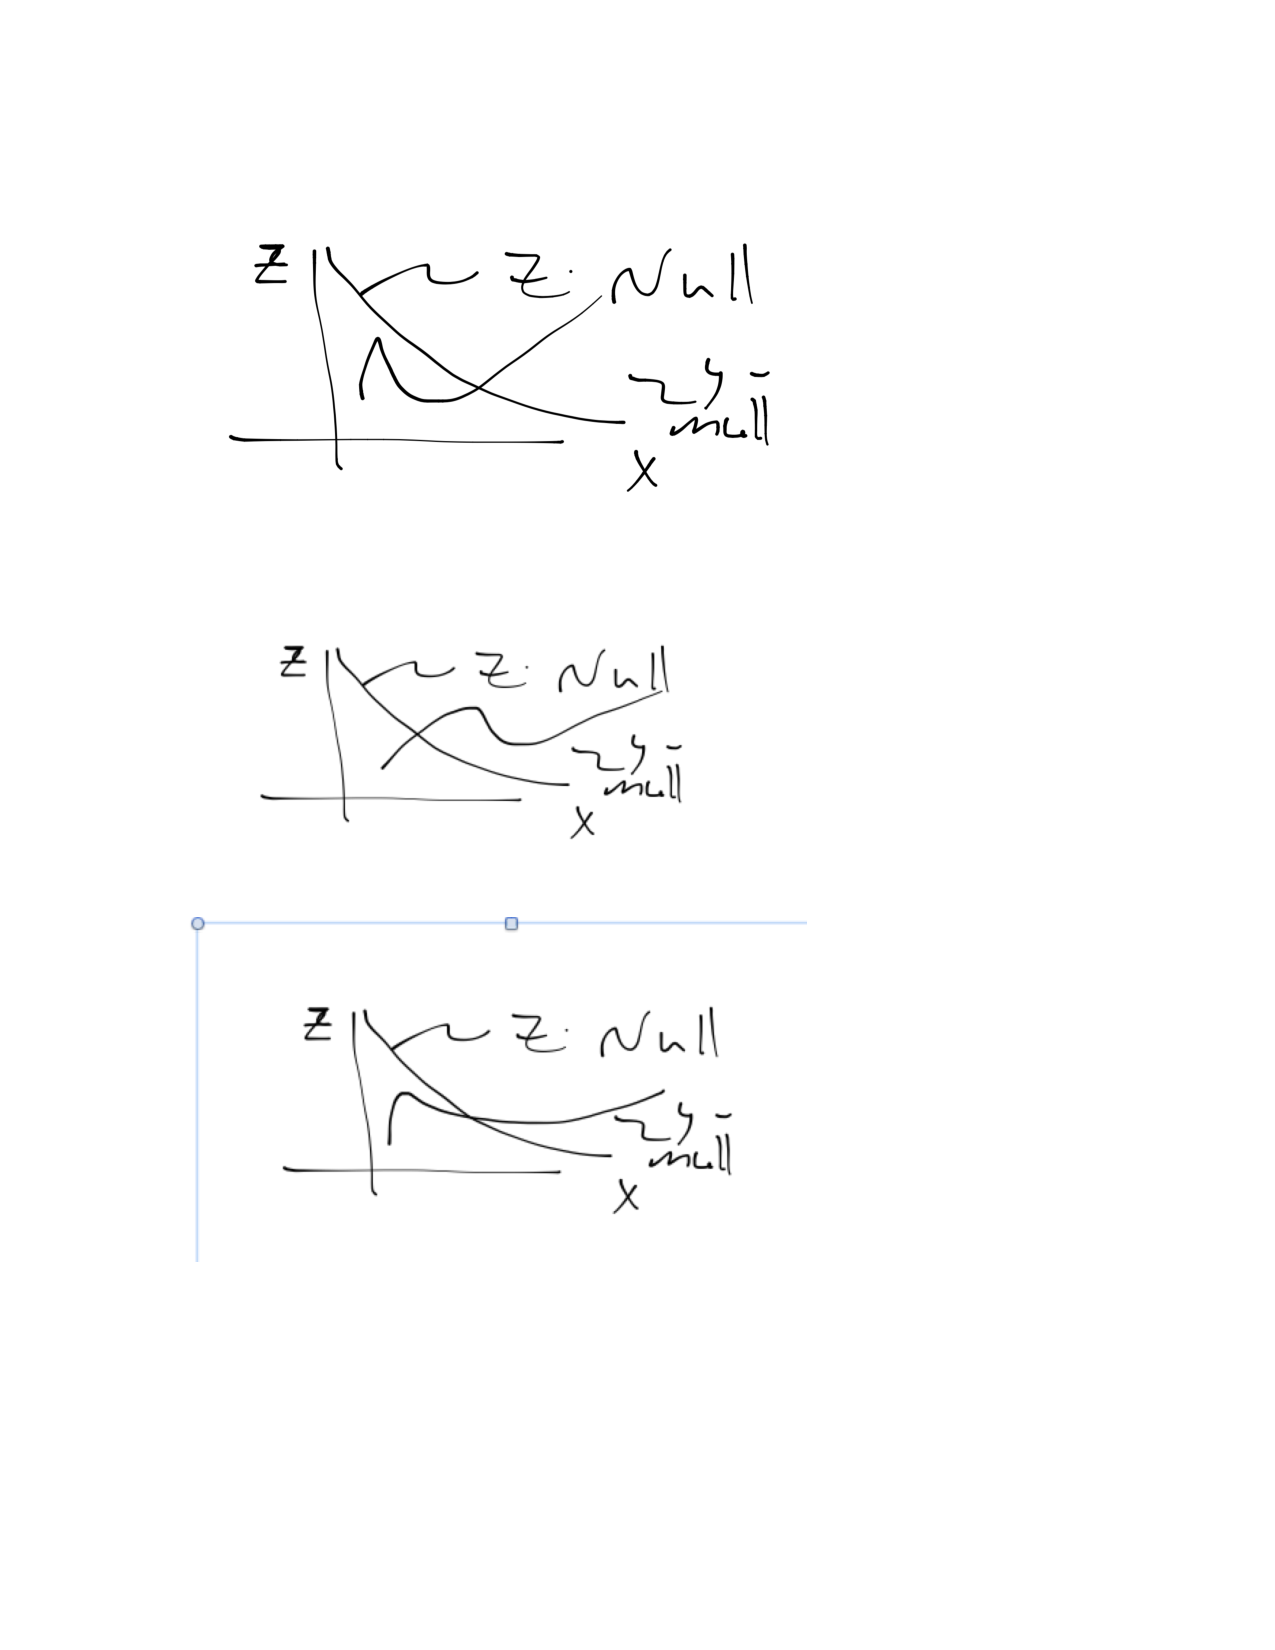
\includegraphics[width=8cm]{figures/bz_3.pdf}
\end{center}
\label{fig:oscper}
\end{figure}
In the last case, where the equilibria is unstable, we should see a limit-cycle and to estimate the period, we need to determine the knee and leading edge as in the van der Pol. 

To get the limits of integration, we find that the points are ...(look in Murray page 272).


\section{Examples of Relaxation Oscillators with Spatial Variation}
\begin{itemize}
\item Threshold waves
\item Wave pulse
\item Threshold behavior in limit cycle regime $\rightarrow$ wave trains.
\item Minimal generic model: $ \lambda - \omega$ oscillator
\end{itemize}
\subsection{Another Model for the BZ Reaction}
Another model for the BZ reaction is given by
\begin{equation}\label{bz2u}
\frac{du}{dt} = Lrv+u(1-u-rv)+u_{xx}
\end{equation}
\begin{equation}\label{bz2v}
\frac{dv}{dt} = -Mv -buv+v_{xx}
\end{equation}
where $u$ and $v$ are chemical reactors. Also,
$$M\sim L=O(10^{-4})$$
$$b\sim O(1)$$
$$5<r<50$$.

The spatially uniform steady states are: $(u,v)=(0,0)$ and $(u,v)=(1,0)$. Since $M$ and $L$ are relatively small, we can neglect them near these equilibria. Setting $M=L=0$:
$$\frac{du}{dt} = u(1-u-rv)+u_{ss}$$
$$\frac{dv}{dt} = -buv+v_{ss}$$.

The steady states of the reduced system are $(u,v)=(1,0)$ and $(u,v)=(0,s)$. The second steady state gives a class of solutions. Essentially  this would be specified when we focused on the wave front and the back.The boundary conditions for the infinite domain are as follows:
$$u(-\infty,t)=0\hspace{0.5in}u(\infty,t)=1$$
$$v(-\infty,t)=1\hspace{0.5in}v(\infty,t)=0$$ Figure~\ref{fig:bz2} shows a plot of $u$ and $v$ against $x$.
\begin{figure}
\caption{$u$ and $v$ satisfying the specified boundary conditions}
\begin{center}
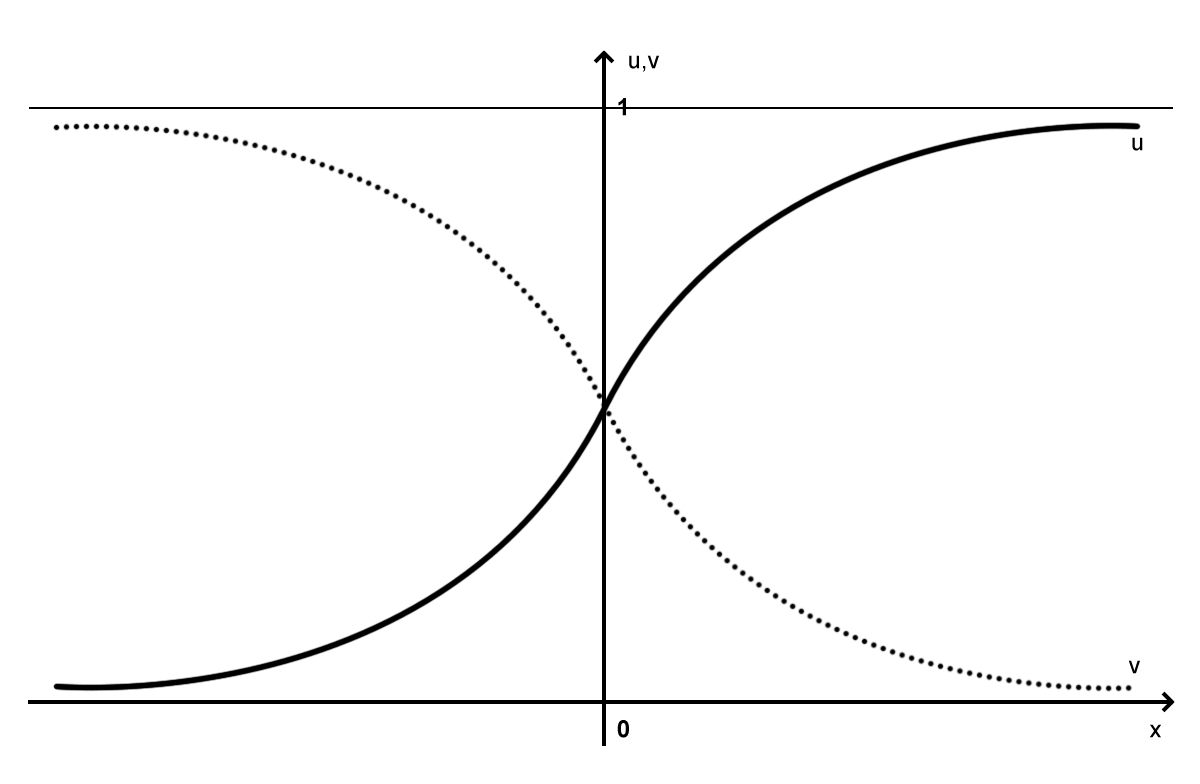
\includegraphics[scale=.20]{figures/BZ_model2.jpg}
\end{center}
\label{fig:bz2}
\end{figure}
\newpage
The goal now is to look for a traveling wave front. We introduce the traveling coordinate $z=x+ct$, and set $u=f(z)$ and $v=g(z)$.
Using this to rewrite the system of PDEs (\ref{bz2u})-(\ref{bz2v}), we obtain

$$f''-cf'+f(1-f-rg)= 0$$
$$g''-cg'-bfg =0$$
$$f(\infty)=g(-\infty)=1$$
$$f(-\infty)=g(\infty)=0$$

As a system, this becomes:
\bea
f_1' &=& f_2 \nonumber \\
f_2' &=& c f_2+f_1(1-rf_1g_1) \nonumber \\
g_1' &=& g_2 \nonumber \\
g_2'&=& cg_2+bf_1g_1 \nonumber
\ena

The steady-states are found when $f_2=0=g_2=0$, $f_1=0$ or $f_1 =$ 
This is a four dimensional system of ODEs, and numerical methods are needed in order to proceed with the analysis and find the wave speed, $c$.

What else can we do?
Look for special cases: if we restrict $v=\frac{1-b}{r}(1-u)$ we obtain a Fisher-like model:
$$
u_t = bu(1-u)+u_{ss}$$

and we can do some more work....
\subsection{Spatiotemporal Fitzhugh-Nagumo Model}
The general Fitzhugh-Nagumo model with spatial diffusion is given by

\begin{equation}\label{fnu}
\cfrac{du}{dt} = f(u)-v+Du_{xx} 
\end{equation}
\begin{equation}\label{fnv}
\cfrac{dv}{dt} = bu - \gamma v
\end{equation}
where $f(u)=u(a - u)(u - 1)$ (Murray, Volume II, p.42).

The spatially homogeneous system ($u_{xx}=0$) has 3 steady states: $(u,v)=(0,0)$, $(u,v)=(1,0)$, $(u,v)=(a,0)$, and exhibits threshold behavior. Figure~\ref{fig:fn} shows the steady states together with the $u$ and $v$ nullclines and the course of some trajectories for the case when the nullclines intersect in just one place. The green curve represenets sub-threshold behavior, and the red curve represents a large pulse as shown in Figure~\ref{fig:wp}. 

To show the existence of travelling pulse solutions for the system with diffusion, we introduce the traveling  coordinate $z=x-ct$. Using the traveling coordinate to rewrite system (\ref{fnu})-(\ref{fnv}), we get

\begin{equation}\label{tcf}
Du'' + c u' + f(u) - v = 0
\end{equation}

\begin{equation}
c v' + b u - \gamma v = 0
\end{equation}

\begin{center}
$\begin{array}{l c l}
u \rightarrow 0, & u' \rightarrow 0, & $as $ z \rightarrow \pm \infty \\
 & v \rightarrow 0, & $ as $ z \rightarrow \pm \infty \\
\end{array} $
\end{center}

A pulse wave, as we see in Figure~\ref{fig:wp}, has a front and a back. We will first just look at how fast the front moves. This requires the assumption $b\sim\gamma\ll1$. If we set $b=\gamma=0$, we get that $v=constant=\overline{v}$. So, equation (\ref{tcf}) becomes

$$Du''+cu' +f(u)-\overline{v}=0$$

and the wave speed, $c$, can be found using 
$$\int u'(Du''+cu'+f(u)-\overline{v})\,dz=0$$

There are regions, where $u$ changes rapidly while $v$ does not, and vice versa. This is a "fast-slow" system.
If $b, \gamma = O(\epsilon)$, i.e. $b = \epsilon M$, $\gamma = \epsilon L$, then a leading order approximation
gives us

\begin{center}
$\begin{array}{l l l}
c v' = & \epsilon [L v - Mu ] & \sim 0 \\
V = & const = & 0\\
\end{array} $
\end{center}

\begin{equation}
c = \left(\cfrac{D}{2} \right)^{1/2}(1 - 2 a)
\end{equation}


This is the bi-stable equation. So, there is a speed $c$ for this equation. If $a = 1/2,$ then we get a standing wave. The
wave speed for the back of the wave is (where $V\approx v_D$)

\begin{equation}
c = \left(\cfrac{D}{2} \right)^{1/2}(u_c - 2u_p + u_D)
\end{equation}

\begin{figure}
\caption{Phase plane for the spatially homogeneous Fitzhugh-Nagumo model}
\begin{center}
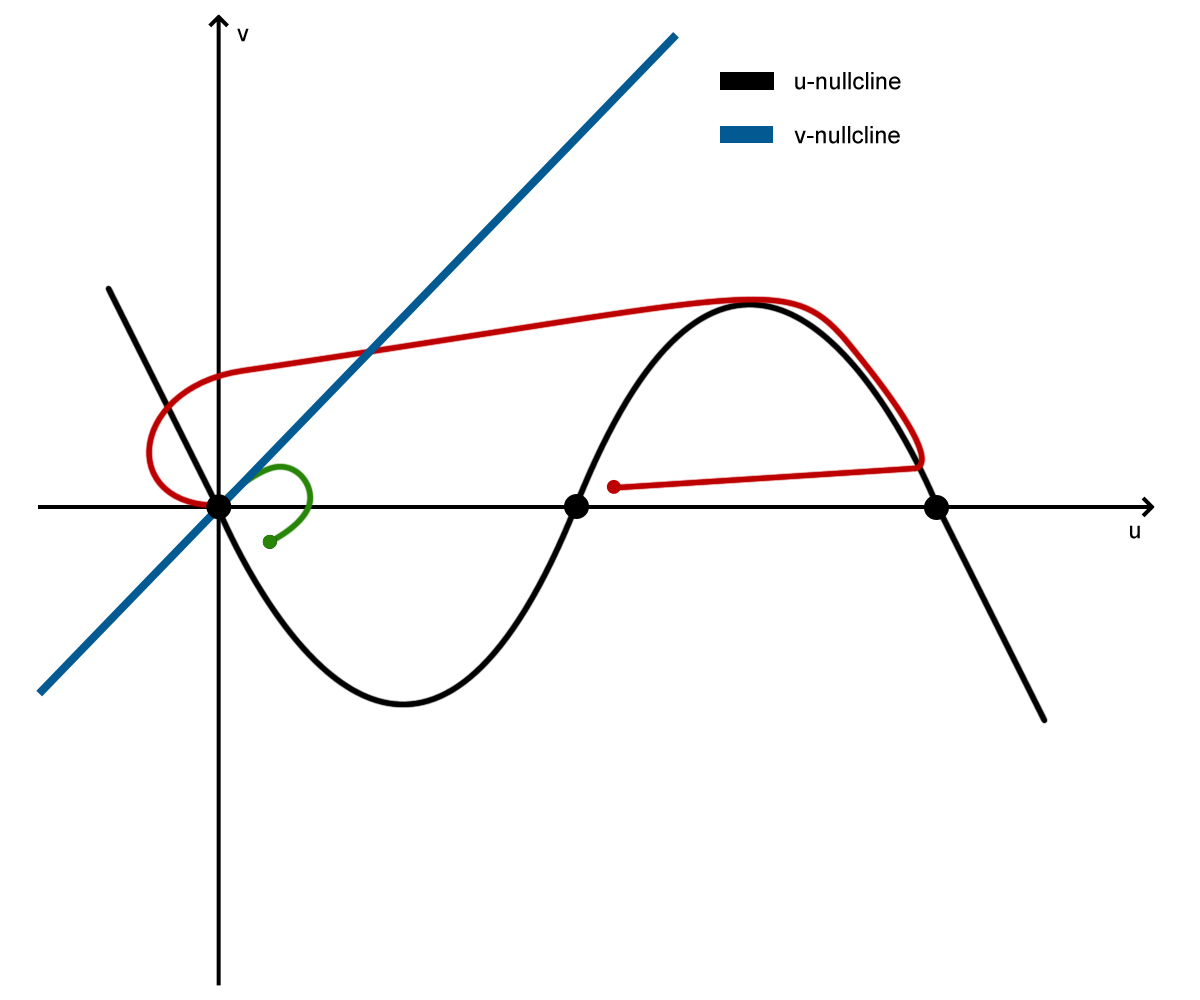
\includegraphics[scale=.20]{figures/FN_figure.jpg}
\end{center}
\label{fig:fn}
\end{figure}

\begin{figure}
\caption{Wave pulse in $z$ space}
\begin{center}
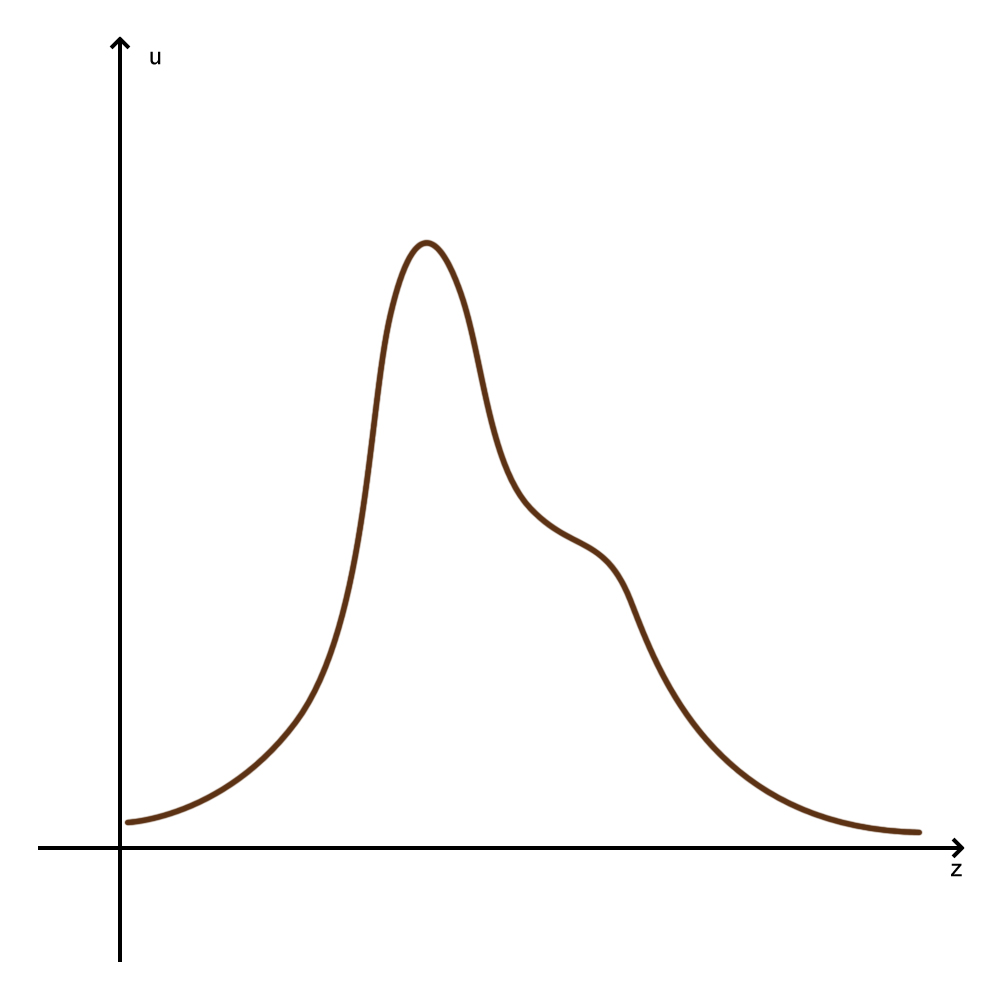
\includegraphics[scale=.20]{figures/Wave_pulse.jpg}
\end{center}
\label{fig:wp}
\end{figure}

\newpage
\section{Wave Trains}

In general, we've been interested in things that look like

$$\vec{u}_t=f((\vec{u}))+D\Delta\vec{u}$$

\noindent Where $$D=
\begin{bmatrix}
d_1 & 0\\
0 & d_2
\end{bmatrix}$$


\noindent We will look for limit cycles in the $\lambda-\omega$ system to get wave trains.

$$\vec{F}(u) =
 \begin{bmatrix}
\lambda(r) & -\omega(r) \\
\omega(r) & \lambda(r)
\end{bmatrix}
\begin{bmatrix}
u \\
v
\end{bmatrix}$$\

\noindent Where $r^2=u^2+v^2$, and there $\exists$ $r_0$ $st$ $\lambda(r_0)=0$, so $\lambda'(r_0)<0$.  In addition, $\omega(r_0)\neq 0$.
Using these conditions guarantees limit cycle oscillations.

\subsection{Original Version of the Lambda-Omega System}
We are only looking at the spatially homologous case (the kinetics).

$$\begin{bmatrix}
u_t \\
v_t
\end{bmatrix} =
 \begin{bmatrix}
\lambda(r) & -\omega(r) \\
\omega(r) & \lambda(r)
\end{bmatrix}
\begin{bmatrix}
u \\
v
\end{bmatrix}$$
Where $r^2=u^2+v^2$.
We make a few assumptions regarding the dependence on $r$. We assume that $\lambda$ is positive if $0\leq r \leq r_0$ and negative if $r>r_0$. This implies that $\lambda(r_0)$ is zero if $\lambda$ is smooth. We assume that $\omega$ is positive.

If we define $c=u+iv$, then we can derive a differential equation for $c$:
\bea
\dt{c} = [\lambda(|c|) + i \omega(|c|)]c\nonumber
\ena
 Even better, if you multiply the first eqn above by $u$ and the second by $v$ and add, you find that
 
 \bea
 \dt{|c|}=\lambda(|c|)|c|
 \ena which implies that $|c| \rightarrow r_0$
\noindent 


\subsection{Complex Version of the Lambda-Omega system}

Here we define the $\lambda-\omega$ system using complex numbers.

$$\frac{dc}{dt}=[\lambda(|c|)+i\omega(|c|)]c$$

\noindent If $\lambda'(r_0)<0$ then the limit cycle is stable. $|c|=r_0$ is that stable equilibrium.

\subsection{The Lambda-Omega System with Diffusion}

We can also look in polar coordinates: $c=u+iv = re^{i\theta}$ and we find that
\bea
\dt{r} &=& r\lambda(r) \nonumber \\
\dt{\theta} &=& \omega(r) \nonumber
\ena
the limit cycle solution is $r=r_0$ and $\theta = \omega(r_0) t + \theta_0$. \\




\noindent If we go back and add diffusion to our system we have

$$\begin{bmatrix}
u_t \\
v_t
\end{bmatrix} =
 \begin{bmatrix}
\lambda(r) & -\omega(r) \\
\omega(r) & \lambda(r)
\end{bmatrix}
\begin{bmatrix}
u \\
v
\end{bmatrix} +D\parxx{}
\begin{bmatrix}
u\\
v
\end{bmatrix}$$

\noindent With $u=r\cos\theta$ and $v=r\sin\theta$.

\noindent When we separate out the matrix into two equations we get.

\bea
\part{r}&=&r\lambda(r)+r_{xx}-r\theta_x^2 \nonumber\\
\part{\theta}&=&\omega(r)+\frac{(r^2\theta_x)_x}{r^2}\nonumber
\ena

\noindent We only changed to polar coordinates for the dependent variables, but leaving the independent variables $x$ and $y$. In addition, if $r$ and $\theta$ are spatially independent, then we get a limit cycle solution.

\begin{center}
$r=r_0$,\hspace{0.25in}$\theta=\theta_0+\omega(r_0)t$
\end{center}

\noindent Look for waves in $t$, $x$ variables. Let $r=\alpha$ and $\theta=t\sigma-kx$ find that for a traveling wave, we must have (same sort of arguments that we looked at before - but crazy messy and found in Kopell's work)

\begin{center}
$\sigma=\omega(\alpha)$,\hspace{0.25in}$k^2=\lambda(\alpha)$
\end{center}

\begin{center}
$\Rightarrow c=\frac{\sigma}{k}$ where c is the wave speed.
\end{center}

Going back in to $u$ $v$ notation we have a one parameter family of periodic solutions: 
\bea
u &=& \alpha\cos(\omega(\alpha)t-x\lambda^{1/2}(\alpha)) \nonumber \\
v&=& \alpha\sin(\omega(\alpha)t-x\lambda^{1/2}(\alpha)) \nonumber 
\ena

Take home: Wave trains (periodic solutions in traveling wave coordinates) exist near the hopf bifurcation.


\newpage
\section{Spiral Waves}

$$\frac{\partial\vec{u}}{\partial t}=\vec{f}(\vec{u})+D\Delta\vec{u}$$

For travelling waves, we let $\vec{u}(x,t)$ look like $\vec{u}(\vec{x}-ct)$ where we had plane waves, but now we have a constant concentration curve. We need a new transformation for spiral waves. Start with a given assumption of the wave form, the derive the wave forms in general from the eikonal-curvature equation.

\subsection{Finding Spiral Wave Coordinates}
Example of a simple spiral wave coordinate:
This part is stupid - just plot a few
Let $\vec{u}(\vec{x},t)=\vec{u}(\phi)$ where $\phi=\Omega t \pm m\theta+\psi(r)$ .
How do we understand this? Set $\phi=0$ and ignore the time dependence:
\bea
\theta = \Psi(r)/m
\ena and $m$ gives the arms of the spiral  (since it divides up the periodic variable $\theta$ and we would see each one if we considered different values of $\phi$.)

 if $m=1$ and $\Psi=ar$ we have the Archimidean sprial. If $m=1$ and $\Psi = a\ln(r)$ we get a logirithmic sprial.
and let $m<0$. Now, look at $\phi$ equal to a constant and freeze time.

$$\frac{\partial\phi}{\partial\theta}=0=\frac{\partial\phi}{\partial\theta}+\frac{\partial\phi}{\partial r}\frac{\partial r}{\partial\theta}$$

Solve for \begin{equation}
	\frac{dr}{d\theta}=\frac{-\phi_\theta}{\phi_r}=\frac{m}{\psi(r)}
\end{equation}

Now, solve the ODE $\Rightarrow \psi'(r)dr=md\theta$

\begin{equation}
	\psi(r)=m\theta+k \rightarrow r=r(\theta)
\end{equation}
When we plot our solution, we get a spiral wave when $\phi$ is a constant value.

\noindent Example. Let $\psi(r)=ar$, $t=0$, $m<0$

$$\phi=m\theta+ar$$

...again let $\phi=$ constant, then

$$\frac{dr}{d\theta}=\frac{m}{a}$$

$$r=\frac{m}{a}\theta+k$$

We have an Archimedian Spiral. (Note: if $m>0$, the spiral spins in the opposite direction)

\noindent Example. Let $\psi(r)=aln(r)$, $t=0$, $m<0$

$$\phi=m\theta+aln(r)$$

...again let $\phi=$ constant, then

$$\frac{dr}{d\theta}=\frac{m}{\frac{(a)}{r}}=\frac{mr}{a}$$

$$r=e^{\frac{m}{a}\theta}$$

We have a spiral with exponential growth.

\subsection{The Lambda-Omega System in Spiral Coordinates}

Now we will do the calculations for the $\lambda-\omega$ system with spiral coordinates.

$$\frac{\partial}{\partial t}
\begin{bmatrix}
u \\
v
\end{bmatrix} =
 \begin{bmatrix}
\lambda(A) & -\omega(A) \\
\omega(A) & \lambda(A)
\end{bmatrix}
\begin{bmatrix}
u \\
v
\end{bmatrix} +D\Delta
\begin{bmatrix}
u\\
v
\end{bmatrix}$$

Where $A^2=u^2+v^2$ which is the magnitude of the concentration or the radius in $(u,v)$ space.  We are using $A$ now to reserve $r$ for the spiral coordinates.  We need to trade in the independent variables $(t,x,y)$ in for the new spiral coordinates (dependent variables: $u$, $v$).

\noindent We let $z$ be a complex number where $z=u+iv$ and replace all
$\begin{bmatrix}
u\\
v
\end{bmatrix}$
vectors with z and get

\begin{equation}
	z_t=(\lambda+i\omega)z+D\Delta z
\end{equation}

This looks like $y_t=Ay+y_{xx}$, the parabolic equation. From this, we can make a guess that the solution might be exponential.


\noindent Let $z=Ae^{i\phi}$ and plug into (42). Since both $A$ and $\phi$ depend on $t$ and $\vec{x}$ we get

\begin{equation}
	A_te^{i\phi}+Aie^{i\phi}\phi_t=(\lambda+i\omega)Ae^{i\phi}+D[-|A\nabla\phi|^2+\nabla^2A]e^{i\phi}+iDA[2\frac{\nabla A\nabla\phi]}{A}+\nabla^2\phi]e^{i\phi}
\end{equation}

\noindent Now equate the real and imaginary parts and get

\begin{equation}
	A_t=A\lambda(A)-DA|\nabla\phi|^2+D\nabla^2A
\end{equation}
and
\begin{equation}
	\phi_t=\omega(A)+2D\frac{\nabla A \nabla\phi}{A}+D\nabla^2\phi
\end{equation}

\noindent We can make another assumption that $A=A(r)$, so $A_t=0$, and $\phi=\Omega t+m\theta+\psi(r)$ and get

\begin{equation}
	DA''+\frac{D}{r}A'+A[\lambda(A)-D\psi^2-\frac{Dm^2}{r^2}]=0
\end{equation}
and
\begin{equation}
    D\psi''+D(\frac{1}{r}+\frac{2A'}{A})\psi =\Omega-\omega(A)
\end{equation}


%%%% details here%%%%%
Then we can try to solve. If we use $A(r)=a_0r^m$, we get $m$ arm spiral solutions.

\begin{center}
\textbf{Propagating Waves}
\end{center}
\textit{Plane Waves}

We initiate the topic with the following question;

Is there a way to predict the travelling coordinate? -Yes, we need to solve
the \textbf{eikonal-curvature }equation. But it is a HARD PDE to solve.
Therefore, we will derive the PDE by analogy.

\[
\frac{\partial u}{\partial t}=\triangledown .\left( D\triangledown
u\right) +kf
\]
\[
U^{\cdot \cdot }+C_{0}U^{\cdot }+f(U)=0 \ \ \text{(the canonical problem)}
\]
\indent To find plane wave solutions of the second equation above, we
suppose that

\[
u=U(\xi ,t) 
\]
where $\xi =x-ct$ and $u$ is a function of a single variable.
\newline \indent In order to begin, we introduce a general moving coordinate system

\[
x=X(\xi ,\tau ), t=\tau 
\]
and we need to specify $\xi $ and $\tau .$

\indent We start with taking the $i^{th}$ coordinate by using chain rule as
following,

\[
\frac{\partial \cdot }{\partial \xi _{i}}=\frac{\partial \cdot }{\partial
x_{1}}.\frac{\partial x_{1}}{\partial \xi _{i}}+\frac{\partial \cdot }{%
\partial x_{2}}.\frac{\partial x_{2}}{\partial \xi _{i}}+\frac{\partial
\cdot }{\partial x_{3}}.\frac{\partial x_{3}}{\partial \xi _{i}}
\]

\[
=\frac{\partial X_{J}}{\partial \xi _{i}}.\frac{\partial \cdot }{%
\partial x_{J}}\ \ \ \ (\ast )
\]

\[
\frac{\partial \cdot }{\partial \tau }=\frac{\partial \cdot }{\partial t}+%
\frac{\partial \cdot }{\partial x_{1}}.\frac{\partial x_{1}}{\partial \tau }+%
\frac{\partial \cdot }{\partial x_{2}}.\frac{\partial x_{2}}{\partial \tau }+%
\frac{\partial \cdot }{\partial x_{3}}.\frac{\partial x_{3}}{\partial \tau }
\]

\[
=\frac{\partial \cdot }{\partial t}+\frac{\partial X_{j}}{\partial
\tau }.\frac{\partial \cdot }{\partial x_{J}} \ \ \ (\ast \ast )
\]

Invert $(\ast )$ and $(\ast \ast )$, we have that

\[
\left\{
\begin{array}{c}
\frac{\partial \cdot }{\partial x_{i}}=\alpha _{ij}\frac{\partial \cdot }{%
\partial \xi _{j}} \\
\frac{\partial \cdot }{\partial t}=\frac{\partial \cdot }{\partial \tau }-%
\frac{\partial X_{j}}{\partial \tau }\alpha _{jk}\frac{\partial \cdot }{%
\partial \xi _{k}}%
\end{array}%
\right. 
\]

\noindent where the matrix with entries $\alpha _{ij}$ is the inverse of the matrix
with entries $\frac{\partial X_{j}}{\partial \xi _{i}}$ which is the
Jacobian of the coordinate transformation.

We identify te variable $\xi _{1}$ as the coordinate normal to level surface
of $u$, so $\xi _{2}$ and $\xi _{3}$ are the coordinates of the moving level
surfaces. We use a simplifying assumption that $\xi _{1}$ has shorter length
scale than  $\xi _{2}$ and $\xi _{3}.$

Here, we will force the following equation be zero by collecting the
coefficients so we have 
\[
U^{\cdot \cdot }+C_{0}U^{\cdot }+f(U)=0.
\]
\indent Therefore, the equation,

\[
\frac{\partial u}{\partial t}=\triangledown .\left( D\triangledown u\right)
+kf \ \ \
\]

\noindent turned into the following form provided that $D$ is scalar,

\[
0=D\alpha _{ip}\alpha _{iq}\frac{\partial ^{2}u}{\partial \xi _{p}\partial
\xi _{q}}+D\frac{\partial \alpha _{ip}}{\partial x_{i}}.\frac{\partial u}{%
\partial \xi _{p}}-\left( \frac{\partial u}{\partial \tau }-\frac{\partial
X_{J}}{\partial \tau }\alpha _{jk}\frac{\partial u}{\partial \xi _{k}}%
\right) +kf(u) \ \ \ \ \ \ (\ast \ast \ast )
\]

By having the assumption that the spatial scale of variation in $\xi _{1}$
is much shorter than the spatial scale of variation in  $\xi _{2}$ and $\xi
_{3},$ we quantify this by supposing that there is a small parameter $%
\varepsilon $ so that $\alpha _{j1}=O(1)$ while $\alpha _{jk}=O(\varepsilon )
$ for all $j$ and $k\neq 1.$ Also, we assume that for leading order in $%
\varepsilon $, $u$ is independent of $\xi _{2}$ and $\xi _{3}$ and $r.$ If
we take into account the $\varepsilon $ dependence of $\alpha _{ij}$, then \
$(\ast \ast \ast )$ simplifies to,

\[
D\left\vert \alpha \right\vert ^{2}\frac{\partial ^{2}u}{\partial \xi
_{1}^{2}}+\left( D\triangledown \cdot \alpha +\frac{\partial x}{\partial
\tau }\cdot \alpha \right) \frac{\partial u}{\partial \xi _{1}}%
+kf(u)=O(\varepsilon )
\]
where $p=q=1$, the order is $1.$

Thus, we concluded the following Eikonal-curvature equation

\[
\frac{\partial \overrightarrow{X}}{\partial \tau }\cdot \alpha
+D\triangledown \cdot \alpha =kC_{0}
\]

\noindent while requiring $D\left\vert \alpha \right\vert ^{2}=k.$

One of the methods that solves the eikonal-curvature equation is called
level sets which determines the motion of an interface. Introduce a
function $S(\overrightarrow{x},t),$ that indicates function for fronts. That
is, if $S(\overrightarrow{x},t)>0,$ the medium is activated, while if $S(%
\overrightarrow{x},t)<0,$ the medium is in the resting state.

The PDE for $S$ is as follows,

\[
S_{t}=\left\vert \triangledown S\right\vert C_{0}\sqrt{Dk}+D\left\vert
\triangledown S\right\vert \triangledown \cdot \left( \frac{\triangledown S}{%
\left\vert \triangledown S\right\vert }\right) 
\]

If we assume no curvature dependence then we ignore the diffusive term, then
we have

\[
\frac{\partial S}{\partial t}=\left\vert \triangledown S\right\vert C_{0}%
\sqrt{Dk}
\]

If $\overrightarrow{R\text{ }}$ is the level surface of $S$, and if $n$ is
the unit normal vector so that surface at same point, we have the following
equation,

\[
\overrightarrow{R_{t}\text{ }}\cdot \overrightarrow{n}=C_{0}\sqrt{Dk}
\]

\textit{Spatial Patterns and Spiral Waves}

In this part, we wish to determine the spatial patterns that may result. The
most common pattern is created by, and spreads outward from a single source.
A second type of spatial pattern is a spiral wave. The mathematical
discussion of spiral waves centers on the nature o periodic solutions of a
system of differential equations with excitable dynamics spacially coupled by
diffusion. A specific example is the FitzHugh-Nagumo equations with
diffusive coupling in two spatial dimensions,

\[
\left\{
\begin{array}{c}
\varepsilon \frac{\partial v}{\partial t}=\varepsilon ^{2}\triangledown
^{2}v+f(v,\omega ) \\
\frac{\partial w}{\partial t}=g(v,\omega )%
\end{array}%
\right. 
\]

To see the implications of the Eikonal-curvature equation, we suppose that
the spiral interface is a curve $R$ given by

\[
x(r,t)=r\cos (\theta (r)-\omega t)
\]
\[
y(r,t)=r\sin (\theta (r)-\omega t)
\]
we then calculate that

\[
R_{t}=
\begin{bmatrix}
-\omega r\sin (\theta (r)-wt) \\
\omega r\cos (\theta (r)-wt)
\end{bmatrix}
\]
and

\[
\sqrt{1+r^{2}\left( \theta ^{\cdot }\right) ^{2}}\overrightarrow{n}=
\begin{bmatrix}
-\sin (\theta -wt)-r\theta ^{\cdot }\cos (\theta -wt) \\
\cos (\theta -wt)-r\theta ^{\cdot }\sin (\theta -\omega t)
\end{bmatrix}
\]

\noindent so that the Eikonal-curvature equation becomes

\[
c(\omega )\sqrt{1+r^{2}\left( \theta ^{\cdot }\right) ^{2}}\overrightarrow{n%
}=\omega r.
\]

An integration then gives

\[
\theta (r)=\rho (r)-\tan (\rho (r)), \ \ \ \rho (r)=\sqrt{\frac{r^{2}}{%
r_{0}^{2}}-1\text{ }}\ \ 
\]
\noindent where $r_{0}\ =\frac{c}{\omega}.$
So the interface is given by

\[
X=r_{0}\cos (s)+r_{0}\rho (r)\sin (s)
\]

\[
Y=r_{0}\sin (s)+r_{0}\rho (r)\cos (s)
\]
where $s=\rho (r)-\omega r.$ This interface is the involute of a circle of
radius $r_{0}.$

\newpage
\section{Local Analysis for PDEs}

\newpage
\section{Turing Systems Analysis} % By Sarah Kim
Turing (1952) suggested that, under certain conditions, chemicals can react and diffuse in such a way as to produce steady state heterogeneous spatial patterns of chemical or morphogen concertration. Thus, Turing systems have been used to study pattern formations in several biological organisms.

\subsection{Turing Criteria}
Turing systems are systems of two PDE reaction-diffusion equaitons that generate patterns. Let $u(x,t)$ and $v(x,t)$ be the concentrations at position $x$ and time $t$ of an activator morphogen and an inhibitor morphogen, respectively.
\begin{equation} \label{Turing1}
\frac{\partial{u}}{\partial{t}}=f(u,v)+d_u\triangle{u}
\end{equation}
\begin{equation} \label{Turing2}
\frac{\partial{v}}{\partial{t}}=g(u,v)+d_v\triangle{v}
\end{equation}
where $f(u,v)$ and $g(u,v)$ are the reaction kinetics and $d_u, d_v > 0$ are the diffusion constants for the activator and inhibitor, respectively. the system of equations (49) and (50) is called a '\textit{Turing system}'. There is criteria that is called '\textit{Turing criteria}'. When the following Turing criteria holds, it generates spatially inhomogeneous patterns.

\textbf{Turing criteria}
\underline{First Turing Criterion} - The system tends to a linearly stable uniform steady state in the absence of diffusion.
\underline{Second Turing Criterion} - The system is unstable in the presence of diffusion. (i.e., Diffusion-driven instability)

\subsection{Linear Stability Analysis for Turing Conditions}
We can use linear stability analysis to derive mathematical conditions that are called '\textit{Turing conditions}' stating when the two Turing criteria are satisfied. We can make the Turing system be non-dimensionalized as following:
\begin{equation} \label{Turing1_1}
\frac{\partial{u}}{\partial{t}}=\gamma f(u,v)+\triangle{u}
\end{equation}
\begin{equation} \label{Turing2_2}
\frac{\partial{v}}{\partial{t}}=\gamma g(u,v)+d\triangle{v}
\end{equation}
where $\gamma > 0$ is proportional to the domain scale, $f(u,v)$ and $g(u,v)$ are the reaction kinetic equations, and $d=\frac{d_v}{d_u} > 1$ is the ratio of diffusion coefficients.
\subsubsection{First Turing Criterion: Linear Stability in the Absence of Diffusion}
Suppose the system of equations (51) and (52) has zero flux boundary conditions (i.e., not be influenced by external input), given initial conditions, and a steady state at $(u_0, v_0)$. Define
$$\textbf{w}=\begin{bmatrix}
u(t)-u_0\\
v(t)-v_0
\end{bmatrix}
=\begin{bmatrix}
\epsilon_u\\
\epsilon_v
\end{bmatrix}$$
where $0 < |\epsilon_u|, |\epsilon_v| < |\epsilon| << 1$, to be a perturbation from the steady state $(u_0, v_0)$. Without diffusion (i.e., a spatially uniform steady state), the system of equations (51) and (52) becomes
$$\begin{bmatrix}
u_t\\
v_t
\end{bmatrix}
=\begin{bmatrix}
\gamma f(u,v)\\
\gamma g(u,v)
\end{bmatrix}$$
Thus,
\begin{equation}\textbf{w}_t=\begin{bmatrix}
u_t\\
v_t
\end{bmatrix}
=\begin{bmatrix}
\gamma f(u,v)\\
\gamma g(u,v)
\end{bmatrix}
=\begin{bmatrix}
\gamma f(u_0+\epsilon_u,v_0+\epsilon_v)\\
\gamma g(u_0+\epsilon_u,v_0+\epsilon_v)
\end{bmatrix}\end{equation}
A Taylor expansion of $u_t$ about the steady state gives
$$u_t=\gamma(f(u_0,v_0)+\epsilon_u f_u(u_0,v_0)+\epsilon_v f_v(u_0,v_0)+O(\epsilon^2))$$
Since $(u_0,v_0)$ is a steady state of the system, $f(u_0,v_0)=0$. Thus,
$$u_t \approx \gamma(\epsilon_u f_u(u_0,v_0)+\epsilon_v f_v(u_0,v_0))$$
In the same way,
$$v_t \approx \gamma(\epsilon_u g_u(u_0,v_0)+\epsilon_v g_v(u_0,v_0)).$$
Thus, the system (53) can be written as
\begin{equation}
\textbf{w}_t=\gamma A \textbf{w}
\end{equation}
where $$A=\begin{bmatrix}
f_u & f_v \\
g_u & g_v
\end{bmatrix}_{(u_0,v_0)} $$
The equation (54) implies that
\begin{equation}
\textbf{w}=ce^{\lambda t}
\end{equation}
for some $\lambda$ to be determined and some constant $c$.
\\
For linear stability in the absence of diffusion, it must be that $w$ approaches to $0$ as $t$ approaches to $\infty$, which occurs when $Re(\lambda) < 0 $. Substituting equation (55) into equation (54) yields
\begin{equation}
c\lambda e^{\lambda t}=\gamma A ce^{\lambda t}
\end{equation}
Dividing equation (56) by $ce^{\lambda t}$ to get the characteristic polynomial
$$det(\gamma A - \lambda I)=0.$$ So, the characteristic polynomial can be rewritten as following:
\begin{equation}
\lambda^2 - \gamma(f_u + g_v)\lambda + \gamma^2(f_u g_v - f_v g_u)=0
\end{equation}
with $f_u, f_v, g_u, g_v$ representing $f_u(u_0,v_0), f_v(u_0,v_0), g_u(u_0,v_0), g_v(u_0,v_0)$, respectively. Thus, it can be solved for $\lambda$ and the following is the result.
\begin{equation}
\lambda_{1,2} = \frac{\gamma}{2}((f_u+g_v)\pm\sqrt{(f_u+g_v)^2-4(f_u g_v - f_v g_u)})
\end{equation}
Then $Re(\lambda) < 0$ follows when
\begin{equation}
Tr(A) = f_u + g_v < 0
\end{equation}
\begin{equation}
Det(A) = f_u g_v - f_v g_u > 0
\end{equation}
which are the two mathematics conditions required to satisfy the first Turing criterion.
\subsubsection{Second Turing Criterion: Instability in the presence of diffusion}
Defining $$D=\begin{bmatrix}
1 & 0 \\
0 & d
\end{bmatrix},$$ the system (51), (52) can be linearized about the steady state $(u_0, v_0)$ to yield \begin{equation}
\textbf{w}_t = D\triangle{\textbf{w}}+\gamma A \textbf{w}
\end{equation}
With the separation of variable technique, the solution to equation (61) can be written as following:
\begin{equation}
c\lambda e^{\lambda t}\textbf{X} = c e^{\lambda t}D\triangle{\textbf{X}}+c e^{\lambda t}\gamma A \textbf{X}.
\end{equation}
Dividing by $ce^{\lambda t}$ and rearranging yields
\begin{equation}
\triangle{\textbf{X}} + D^{-1}(\gamma A - \lambda I)\textbf{X} = 0.
\end{equation}
The above equation (63) is of the form of a Helmholtz equation, $\triangle{\textbf{X}}+k^2 \textbf{X}=0$, an eigenvalue problem with eigenfunctions $\textbf{X}_n$ and their associated eigenvalues $k_n$, where
\begin{equation}
k^{2}_{n} I = D^{-1}(\gamma A - \lambda I).
\end{equation}
Thus, the complete solution to equation (61) is
\begin{equation}
\textbf{w}(x,t)=\sum_n{c_n e^{\lambda t} \textbf{X}_n(x)}.
\end{equation}
To get diffusion-driven instability, $\lambda$ must satisfy $Re(\lambda) > 0$. Equation (64) implies that
$$|\lambda I - \gamma A + Dk^2|=0,$$ which can be rewritten as
$$\lambda^2 + \lambda[k^2(1+d)-\gamma(f_u + g_v)]+h(k^2)=0,$$ where
$$h(k^2)=dk^4-\gamma(df_u+g_v)k^2+\gamma^2|A|.$$
This can be solved for $\lambda$ with the quadratic formula, yielding roots
\begin{equation}
\lambda_{1,2}=\frac{1}{2}(-( k^2(1+d)-\gamma(f_u+g_v))\pm \sqrt{(k^2(1+d)-\gamma(f_u+g_v))^2-4h(k^2)}).
\end{equation}
To satisfy $Re(\lambda) > 0,$ either
\begin{equation}
k^2(1+d)-\gamma(f_u+g_v) < 0
\end{equation}
or
\begin{equation}
\lambda=\frac{1}{2}(-( k^2(1+d)-\gamma(f_u+g_v))+
\sqrt{(k^2(1+d)-\gamma(f_u+g_v))^2-4h(k^2)})
\end{equation}
and
\begin{equation}
h(k^2) < 0.
\end{equation}
Since $\gamma, d > 0$ by definition and $f_u + g_v < 0$, then the equation (67) cannot be satisfied if the first Turing criterion is to be satisfied as well. Thus, in order to satisfy the second Turing criterion, the equation (68) and (69) must hold. Thus,
\begin{equation}
df_u + g_v > 0.
\end{equation}

Since $f_u+g_v<0$ it must be that $d\neq1$ and that $f_u$ and $g_v$ have different signs.
Typically, $f_u > 0, g_v < 0.$ \\
$d > 1$ for instability or diffusion coefficient of v $>$ diffusion coefficient of u.
\subsection{Particular Turing System}
Turing-Gierer-Meinhardt created a solution to the pattern formation problem that during development a pattern is formed in a practically featureless domain.  They constructed pattern-generating chemical reactions where there is an activator and an inhibitor which is sufficient to create biological patterns.

\subsubsection{Basic Activator-Inhibitor Model}
Let $a$ be an activator and $h$ be an inhibitor that are produced by cells with density $\rho_a, \rho_h$ respectively.

Inhibitor produce rate $C_h a^2/cell$.
Activator produce rate $C_a/cell$ but is affected by inhibior and activator if $a >> 1$.
Activator Rate $= C_a + ca^2/h$.

Assume linear decay and the model is
$$a_t=\rho_a(C_a+ca^2/h)-\mu_a a + D_a a_{xx}$$
$$h_t=\rho_h C_h a^2 - \mu_h h + D_h h_{xx}$$
Where $D$ represents the diffusivities; $\mu$ is the decay rates, and $C$ represents some constant.

\noindent After the equations are non-dimensionalized have
$$\frac{\partial A}{\partial t}=1+R\frac{A^2}{H}-A+A_{ss}$$
$$\frac{\partial H}{\partial t}=Q(A^2-H)+PH_{ss}$$

Where

\begin{center}
 $P=\frac{D_h}{D_a}$, \hspace{0.2in}$R=\frac{C\mu_h}{c_ac_h\rho_h}$
\end{center}

\begin{center}
 $Q=\frac{\mu_h}{\mu_a}$, \hspace{0.2in}$s=\frac{x}{\sqrt{D_a/\mu_a}}$
\end{center}

\noindent 1) Look spatially homogeneous states

Setting the non-dimensionalized equations equal to zero (exculding the spatial part) get
\begin{center}
$1+R\frac{A^2}{H}-A=0$, \hspace{0.2in} $Q(A^2-H)=0$
\end{center}
$$H=A^2 \Rightarrow  \hspace{0.2in} 1+R-A=0 \Rightarrow \hspace{0.2in} \bar{A}=1+R, \hspace{0.12in} \bar{H}=(1+R)^2$$

\noindent 2) Check for temporal stability

First, need the Jacobian
$$J=
\begin{bmatrix}
f_A&   f_h\\
g_a &   g_h
\end{bmatrix}$$

Evaluated at $\bar{A}$ and $\bar{H}$ get
$$J=
\begin{bmatrix}
(R-1)/(R+1)&    -R/(1+R)^2\\
2Q(1+R) &   -Q
\end{bmatrix}$$
 we must have that $\frac{R-1}{R+1}<Q$
\noindent 3) Perturb with spatial functions on the infinite domain

$$A'=\hat{A}(\tau)cos(s/l)$$
$$H'=\hat{H}(\tau)cos(s/l)$$

$$\frac{\partial\hat{A}}{\partial\tau}=\left(\frac{R-1}{R+1}-\frac{1}{l^2}\right)\hat{A}-\frac{R}{(1+R)^2}\hat{H}$$
$$\frac{\partial\hat{H}}{\partial\tau}=2Q(1+R)\hat{A}-\left(Q+\frac{P}{l^2}\right)\hat{H}$$

The solutions to these odes decay to zero if and only if

$$-\left(\frac{R-1}{R+1}-\frac{1}{l^2}\right)\left(Q+\frac{P}{l^2}\right)+\frac{2QR}{R+1}>0$$

which reduces to

$$Q+\frac{P}{l^2}-\left(\frac{R-1}{R+1}-\frac{1}{l^2}\right)>0$$

which always holds because $Q>\frac{R-1}{R+1}$.

Now we multiply by $l^2$ and rearrange to get the stability condition.

$$Ul^4+\left(U-\frac{R-1}{R+1}\right)l^2+1>0$$

where $U=Q/P$

For \textbf{stability} $F(l^2)>0$ where
$$F(\alpha)=U\alpha^2+\left(U-\frac{R-1}{R+1}\right)\alpha+1$$

and is only true for $U>\frac{R-1}{R+1}$

For \textbf{instability} need $F(\alpha)<0$.  Need two real roots of $F(\alpha)=0$ where at least one is postive for instability.

$$2U\alpha=\frac{R-1}{R+1}-U\pm\sqrt{\left(U-\frac{R-1}{R+1}\right)^2-4U}$$

There are real roots when

$$\left(U-\frac{R-1}{R+1}\right)^2>4U$$

Taking the square root of both sides gives

$$\frac{R-1}{R+1}>2\sqrt{U}+U$$

Since $U$ is positive, with this condition there the roots are positive, so this is the condition for instability.  There

are two ways to satisfy this condition: either $R$ is large or $U$ is small.


\begin{list}{\leftmargin=2em}
\item$\bullet$ For $U$ small, the decay of the inhibitor is larger than the decay of the activator (larger $Q$), or the diffusion of the activator is larger than the diffusion of the inhibitor (smaller P).
\item$\bullet$ For R large, take the limit as $R\rightarrow\infty$
\end{list}
$$1>2\sqrt{U}+U$$
$$U+2\sqrt{U}+1<1+1$$
$$(\sqrt{U}+1)^2<2$$
$$\sqrt{U}<\sqrt{2}-1$$

\indent\indent So the approximate instability condition is
$$\sqrt{U}<0.4\Rightarrow\sqrt{\frac{D_a/\mu_a}{D_h/\mu_h}}<0.4$$

Note: Now the diffusions do not need to be equal.  The ratios of these length scales have to satisfy the inequality.

Particularly, the activator length scale must be less than the inhibitor length scale.

\subsubsection{Critical Wavelength}
What is the critical wavelength where $U$ barely satisfies the instability inequality $$F(l^2)<0$$ if $R>>1$?
$$Ul^4-(1-U)l^2+1<0$$
$$l^2=\frac{1-U\pm\sqrt{(1-U)^2-4U}}{2U}$$

For Real $l^2$ then
$$(1-U)^2>4U$$
$$U^2-6U+1=>0$$
\begin{center}
$U>3+2\sqrt{2}$\hspace{0.1in} or\hspace{0.1in}  $0<U<3-2\sqrt{2}$
\end{center}

The first range does not satisfy $F(l^2)<0$, so using the second range have $l=1+\sqrt{2}=l_c$ when $R\rightarrow\infty$.  This

critical value is the first wavelength that becomes unstable when $u$ is perturbed.


Looking back at the spatial variable $x$

$$cos\left(s/l\right)=cos\left(\frac{x}{l\sqrt{D_a/\mu_a}}\right)$$

We get a critical wavelength $$L_c\approx10\sqrt{D_a/\mu_a}$$

Note that $D_a$ and $\mu_a$ are measurable quantities, so one can make an estimate for what wavelength patterns will

form.

In addition, if given two wavelengths that have the equal lambda values on the dispersion curve neither wins out unless there is a higher concentration for one of the wavelengths.  In that case, the higher concentration value wins out.  Otherwise, the wavelength that wins it the wavelength with the higher lambda value.  For example, if $u'=A_1(t)cos(\omega_1x)+A_2(t)cos(\omega_2x)$
and $\omega_1=\omega_2$ but $A_1>>A_2$ then $\omega_1$ wins.

(figure)


So far this analysis has only be in the infinite domain.  To find the biologically relevant wavelength, this analysis must be done on a finite domain (the perturbations need to satisfy the proper boundary conditions which is an eigenvalue problem).

If there is an initial condition $f(x)$, have

$$A=\Sigma a_ke^{\lambda t}cos(s/k)$$

where this represents all modes and if the modes are added together the initial condition is obtained.

\subsubsection{Non-Linear and Weakly Non-Linear Analysis}
\b{this is out of Segel}
Linear analysis predicts unstable frequencies that grow exponentially (which is not biological).  The non-linear terms temper this exponential growth (the $\epsilon^2$ and higher terms that were ignored in the non-linear analysis).

\noindent To understand how the exponential growth is controlled one can:

\begin{enumerate}
\item run numerical simulations
\item use weakly non-linear analysis
\end{enumerate}

When weakly non-linear analysis is used for the hydra, there is an inhomogeneous steady state in time.  The steady state is a linear combination of harmonics of unstable modes.  This is generally true for many Turing systems.

\noindent The effects if non-linearity:

\begin{itemize}
\item For single-mode perturbations/excitations
\begin{enumerate}
\item self-damping (amplitude damping)
\item generation of harmonics
\item spatial average changes
\end{enumerate}
\item For multi-mode excitation
\begin{enumerate}
\item inter-mode suppression
\end{enumerate}
\end{itemize}

The model for weakly non-linear growth for a single mode is

$$\frac{dA}{dt}=aA-a_1A^3$$

with $a_1>0$ and $a\neq 0$, for this particular model have

$$\frac{dA}{dt}=(a-a_1A^2)A=a\left(1-\frac{a_1}{a}A^2\right)A$$

The non-linear model is $\frac{dA}{dt}=aA$

(figure)

The model for inter-node suppression where $A$ and $B$ are modes is

$$\frac{dA}{dt}=aA-a_1A^3-a_2AB^2$$
$$\frac{dB}{dt}=bB-b_1B^3-b_2BA^2$$

For this model there are four equilibria corresponding to $A=0$, $B=0$, $A=\sqrt{a/a_1}$, and $B=\sqrt{b/b_1}$

(figure)

The $(\sqrt{a/a_1},\sqrt{b/b_1})$ equilibrium represents the coexistence of A and B, but it is an unstable saddle point.  The origin is unstable while the two other equilibria are both stable.  This is a \textbf{competitive exclusion model}.

\subsection{Slime Mold}

There is a biological phenomena demonstrated by cellular slime mold.  When grown in a petri dish, slime mold will exist as independent unicellular organisms until their food source runs out. At this point, the cells will begin attract other cells and they aggregate together. Depending on certain conditions they will create only one large collection or several groupings. At these ``aggregation sites,'' the cells will begin to work together as a collective organism and create a slug-like form with differentiated parts. After this stage, they form a tree/mushroom-like structure that will burst to spread spores of the slime mold.

Slime molds are chemotactic.  They produce cAMP to signal each other (the signal decreases when food is available and increases when food is scarce). The slime mold cells are attracted to the cAMP signal and have a random walk that is biased by the gradient of cAMP.

How do we get the different aggregations? What is the determining factor that allows there to be only one or many aggregation sites?

$a=$ concentration of slime mold
$c=$ concentration of cAMP

$$\frac{\partial a}{\partial t}=-\nabla(J_{random}+J_{chemotactic})$$
$$\frac{\partial c}{\partial t}=sources/sinks(a)-\nabla(J_{diffusive})$$

\indent Here we look at the model presented by Keller and Segel (1970) in 1D.

\begin{equation}
\frac{\partial a}{\partial t}=-\frac{\partial}{\partial x}(-\mu\frac{\partial a}{\partial x}+\chi a\frac{\partial c}{\partial x})
\end{equation}
\begin{equation}
    \frac{\partial c}{\partial t}=-\frac{\partial}{\partial x}(-D\frac{\partial c}{\partial x})+fa-kc
\end{equation}

\indent We need a plus sign inside the parentheses of slime mold concentration equation because this is a chemotactic attractive system, so the change in concentration of the cAMP in space is negative, which increases the slime mold concentration rate in time. We have a non-linear system (due to the $a\frac{\partial c}{\partial x}$ term) of PDES.  Now we must analyze the system.

\indent First Step: find equilibria. Unfortunately, the steady-state is a non-linear ODE, so we will look for a solution uniform in space. $a,c =$ constants in time and space.

\indent\indent Equation (43) is satisfied for $\forall(a,c)$ pairs.

\indent\indent Equation (44) is satisfied if $fa=kc$ or $a=\frac{kc}{f}$.

So, our equilibria are $(0,0)$ and $(\bar{a},\bar{c})$ that satisfy the condition $a=\frac{kc}{f}$.

\noindent Second Step: linearize/perturb the system in time and space.  We will look for solutions that are near the equilibria and the leading order expansion.

$$a=\bar{a}+\epsilon a'(x,t)$$
$$c=\bar{c}+\epsilon c'(x,t)$$

\begin{equation}
	\frac{\partial}{\partial t}(\bar{a}+\epsilon a')=-\frac{\partial}{\partial x}(-\mu\frac{\partial}{\partial x}(\bar{a}+\epsilon a')+\chi(\bar{a}+\epsilon a')\frac{\partial}{\partial x}(\bar{c}+\epsilon c'))
\end{equation}

{\footnotesize
\begin{equation}
\bar{a}_t+\epsilon a^{'}_{t}=-\frac{\partial}{\partial x}(-\mu\bar{a}_x)-\frac{\partial}{\partial x}(-\mu\epsilon a'x)-\frac{\partial}{\partial x}(\chi\bar{a}\bar{c}_x)-\frac{\partial}{\partial x}\epsilon(\chi(a'\bar{c}_x+\bar{a}c'_x))-\epsilon^2\frac{\partial}{\partial x}(\chi a'c'_x)
\end{equation}
}

\begin{equation}
	O(1): \bar{a}_t=-\frac{\partial}{\partial x}(-\mu\bar{a}_x)-\frac{\partial}{\partial x}(\chi\bar{a}\bar{c}_x)
\end{equation}

$\bar{a}$, $\bar{c}$ are constant in time and space, so this equation is satisfied for $\bar{a}_t,\bar{a}_x,\bar{c}_x=0$.

\begin{equation}
	O(\epsilon): a'_t=-\frac{\partial}{\partial x}(-\mu a'_x)-\frac{\partial}{\partial x}(\chi(a'\bar{c}_x+\bar{a}c'_x))
\end{equation}



\indent since $\bar{c}_x =0$ get


\indent $a'_t=-\frac{\partial}{\partial x}(-\mu a'_x)-\frac{\partial}{\partial x}(\chi\bar{a}c'_x)$


\indent If $\epsilon$ is small enough, then the $\epsilon^2$ terms are negligible, so we will ignore them.


\indent(44):$\frac{\partial}{\partial t}(\bar{c}+\epsilon c')=-\frac{\partial}{\partial x}(-D\frac{\partial}{\partial x}(\bar{c}+\epsilon c'))+f(\bar{a}+\epsilon a')-k(\bar{c}+\epsilon c')$

\indent$O(1)$: $\bar{c}_t=-\frac{\partial}{\partial x}(-D\bar{c}_x)+f\bar{a}-k\bar{c}$
\indent since $\bar{c}_t, \bar{c}_x =0$ get
\indent $\bar{a}=\frac{\bar{c}k}{f}$
\indent$O(\epsilon)$: $c'_t=-\frac{\partial}{\partial x}(-D c'_x)+fa'-kc'$

Now we have a linear system for the perturbed variables $a'$ and $c'$.

\begin{equation}
a'_t=\mu a'_{xx}-\chi\bar{a}c'_{xx}
\end{equation}
\begin{equation}
c'_t=Dc'_{xx}+fa'-kc'
\end{equation}\

We can now do a separation of variables.  This is a parabolic system, so we can assume (without boundary conditions) that if we went through the separation of variables we have the following eigenvalue and eigenfunction solutions.

\begin{equation}
a'=Ae^{\lambda t}e^{i\omega x}
\end{equation}
\begin{equation}
c'=Ce^{\lambda t}e^{i\omega x}
\end{equation}\

Now, if we plug (47) and (48) into (45) and (46) we get

$$\lambda Ae^{\lambda t}e^{i\omega x}=-\mu\omega^2Ae^{\lambda t}e^{i\omega x}+\chi\bar{a}\omega^2Ce^{\lambda t}e^{i\omega x}$$
$$\lambda Ce^{\lambda t}e^{i\omega x}=-\omega^2DCe^{\lambda t}e^{i\omega x}+fAe^{\lambda t}e^{i\omega x}-kCe^{\lambda t}e^{i\omega x}$$\

By dividing by $e^{\lambda t}e^{i\omega x}$ get

$$\lambda A=-\mu\omega^2A+\chi\bar{a}\omega^2C$$
$$\lambda C=-\omega^2DC+fA-kC$$\

Now, we rearrange the equations.

$$A[\lambda+\mu\omega^2]+C[-\chi\bar{a}\omega^2]=0$$
$$A[-f]+C[\lambda+\omega^2D+k]=0$$\

Write this as a matrix.

$$\begin{bmatrix}
\lambda+\mu\omega^2 & -\chi\bar{a}\omega^2 \\
-f & \lambda+\omega^2D+k
\end{bmatrix}
\begin{bmatrix}
A\\
C
\end{bmatrix}=
\begin{bmatrix}
0\\
0
\end{bmatrix}$$\

Solve for $(A,C)\neq(0,0)$ (aka finding non-trivial solutions).  As long as the matrix is not invertible then we have non-trivial solutions.  The matrix is non-invertible if the determinant equals zero.

$$(\lambda+\mu\omega^2)(\lambda+\omega^2D-k)+f(\chi\bar{a}\omega^2)=0$$\

So, $\lambda$ will be a function of $\omega, \mu, D, k, f, \chi, \bar{a}$, and we want $\lambda<0$ for stable solutions, and if $\exists\omega$, such that $\lambda>0$ we have unstable solutions.  This corresponds to one and multiple aggregation sites respectively.

For nontrivial solutions we need $\det (J)=0.$

Therefore, 
\[
\left( \lambda +\mu w^{2}\right) \left( \chi +w^{2}D+K\right)-f\chi \overline{a}w^{2}=0
\]
\indent We know that
\[ 
\lambda ^{2}+b\lambda +c=0.
\]
\indent Condition for instability

\[ 
\chi f\overline{a}>\mu \left( K+Dw^{2}\right)  
\]
dispersion relation.
If $w<<0,$ so $\frac{\chi f\overline{a}}{\mu K}>1$ ,which is easier to
satisfy for low $\mu $ and $K$ where $K$ is chemoattractant decay rate.

Increases in $\mu $ and $K$ have stabilizing effect. What about nonlinear
effects?

\textit{a) }Explore numerically

\textit{b)}Look for higher order corrections

\[
 u=\overline{u}+\varepsilon u_{1}+\varepsilon ^{2}u_{2+...}
\]
where $\overline{u}$ is the dominant influence.
or
\[
u=\overline{u}+f_{1}\left( \varepsilon ,\overline{u}\right)
u_{1}+f_{2}\left( \varepsilon ,\overline{u},u_{1}\right) u_{2+...}
\]

\newpage
Nonlinearities,

\textit{1)}Self damper modes

\textit{2)} Generation of harmonics

\textit{3)}Inter mode suppression$\Longrightarrow $competitive exclusion of
modes.



\newpage
\section*{Part II}
\section{Mechanical Models}

\section{Poiseuille Flow}
%\subsection{Field-Noyes Model}

\begin{equation}\label{momentum}
	\frac{\partial \vec{u}}{\partial t} + (\vec{u}\cdot \nabla) \vec{u} = \mu \nabla^2 \vec{u} - \nabla p
\end{equation}

\begin{equation}\label{continuity}
	\nabla \cdot \vec{u} = 0
\end{equation}

Poisuelle Flow can be interpreted as flow in a channel between two horizontal plates. For boundary conditions at $\infty$
in the x-direction, we assume that the solution must be bounded. At $y = 0$ and $y = L$, we apply that there is no flow in
y-direction.  The pressure boundary conditions are "up for grabs" at the wall.

$Ansatz$: assume that the flow is independent of $x$ and $t$.

\[
	\vec{u} = <u(y), v(y)>
\]

>From incompressibility, we have that $u_x + v_y = 0$ and by independence in $x$, we know that $u_x = 0$. This tells
us that $v = const$.  But, we know that there is no vertical flow. If there were, we would have flow at the wall, violating
our boundary conditions. So, we have that $v = 0$. So, we now can simplify Eqn. (\ref{momentum})

\[
	(\vec{u}\cdot \nabla) \vec{u} = u \cdot u_x + v \cdot v_y = 0
\]

Also

\[
	 \mu \nabla^2 \vec{u} - p_x = \mu(u_{xx} + v_{yy}) - p_x= \mu(0 + v_yy) - p_x = 0
\]

So, we are solving the following equation.

\begin{equation}\label{pflow}
u_{yy} = \frac{p_x}{\mu}
\end{equation}

>From Eqn. (\ref{pflow}), we can see that if there is no pressure gradient, then there is no flow, yielding the trivial
solution.  So, let us assume that $p_x$ is independent of $x$, i.e. $p = p_0 x$.  Plugging this into (\ref{pflow}), we
get that we are solving

\[
	u_{yy} = \frac{p_0}{\mu}
\]

This gives us the solution

\begin{equation}\label{pflow_soln1}
u = \frac{p_0}{2 \mu}y^2 + c_1 y + c_2
\end{equation}

With boundary conditions $u(x,0) = u(x,L) = 0$. Apply boundary conditions and solving for the arbitrary constants, we find
the following flow profile.

\[
	u = \frac{p_0}{2 \mu}y (y - L)
\]

\section{Couette Flow}
Shear flow gives a linear speed profile.  \\
Instabilities in Fluids
\begin{enumerate}
	\item Reynolds Instability - goes from laminar flow to turbulent flow
	\item Surface Waves - waves cause when a less viscous fluid travels over a more viscous fluid. Perturbs the
		interface. This is important for ocean waves.
	\item Raleigh(-Benard) Instability. Stratified fluid of two densities, one on top of the other. If bottom fluid is more
		dense, system is stable. If not, this will create buoyancy forces. R.B. does changes in density via heating.
\end{enumerate}

\subsection{Raleigh Instability} Inviscid flow with differing densities. Biologically, one can think of an aerotaxic bacteria
wanting to stay at the top of a tank, creating a biofilm. This causes circulation from the bacteria trying to stay near the surface.

\[
\nabla \cdot \vec{u} = 0
\]

\[
	\frac{D \rho}{Dt} = 0
\]

\[
	\rho \frac{D \vec{u}}{Dt}  = - \nabla p - \rho g \begin{bmatrix}	0\\0\\1	\end{bmatrix}
\]

Performing an appropriate non-dimensionalization, this is transformed to

\[
	\frac{D \vec{u}}{Dt}  = - \nabla p - \rho \begin{bmatrix}	0\\0\\1	\end{bmatrix}
\]

We apply boundary conditions $\vec{u}\cdot \hat{z} = 0$ at $z = 0, d$. Step 1 is to look for special solutions and take
perturbations.  \\
\emph{Special Solution}: $\vec{u} = 0$, $\rho = r(z)$, $p = - \int_0^z r(s)ds$. This satisfies continuity and the momentum
equation.  So, let's take a perturbation.

\begin{equation}
\vec{u} = 0 + \epsilon \vec{u_1}(x,y,z)
\end{equation}

\begin{equation}
\rho = r(z) + \epsilon \rho_1(x,y,z)
\end{equation}

\begin{equation}
p = - \int_0^z r(s)ds + \epsilon p_1(x,y,z)
\end{equation}

\[
\nabla \cdot (\epsilon \vec{u_1}) = 0
\]

\[
\frac{D}{Dt}(r(z) + \epsilon\rho_1) = 0	\rightarrow	\frac{\partial}{\partial t} (r + \epsilon \rho_1) + (\epsilon \vec{u_1} \cdot \nabla)(r + \epsilon\rho_1) = 0
\]

\[
\frac{D}{Dt}(\epsilon \vec{u}) = - \nabla (- \int_0^z r(s)ds + \epsilon p_1 ) - \left(r(z) + \epsilon p_1 \begin{bmatrix}0\\0\\1 \end{bmatrix}\right)
\]

Taking only the first order terms from the second equation, we get
\[
\epsilon \left( \frac{\partial\rho_1}{\partial t} + (\vec{u_1} \cdot \nabla)r	\right) = 0
\]

Collecting all of our equations, we have the following.

\begin{equation}\label{c_cont}
\nabla \cdot \vec{u_1}
\end{equation}

\begin{equation}\label{c_rho}
\frac{\partial \rho_1}{\partial t} + r'(z)w_1 = 0
\end{equation}

\begin{equation}\label{c_u}
r(z)\frac{\partial u}{\partial t} + (p_1)_x = 0
\end{equation}

\begin{equation}\label{c_v}
r(z)\frac{\partial v}{\partial t} + (p_1)_y =0
\end{equation}

\begin{equation}\label{c_w}
r(z)\frac{\partial w}{\partial t} + (p_1)_z + \rho_1 =0
\end{equation}

We will assume a solution of the form

\[
\begin{bmatrix} u_1 \\ v_1 \\ w_1 \\ p_1 \\ \rho_1 \end{bmatrix} = \begin{bmatrix} U(z) \\V(z)\\ W(z)\\P(z) \\ R(z) \end{bmatrix} e^{\sigma t + i (k_1 x + k_2 y)}
\]

From (\ref{c_cont})
\[
ik_1 U + ik_2 V + W' = 0
\]

From (\ref{c_rho})
\[
\sigma R + r'(z)W = 0
\]

From (\ref{c_u})
\[
\sigma r(z) U + i k_1 P = 0
\]

From (\ref{c_v})
\[
\sigma r(z) V + i k_2 P = 0
\]

From (\ref{c_w})
\[
\sigma r(z) W + P'(z) + R = 0
\]

From the third and fourth equations, one can solve for $U$ and $V$, then substitute into the first equation.

\[
\frac{P}{\sigma r} k^2 + W' = 0
\]

Where $k = k_1^2 + k_2^2$. So,

\[
P = \frac{r \sigma}{k^2}W'	\quad \rightarrow \quad P' = (\frac{r \sigma}{k^2}W')'
\]

The, we can see that $R = -\frac{1}{\sigma} r' W$, and so

\[
(r(z)W')' + k^2(\frac{1}{\sigma}r' - r)W = 0,	\quad \quad W(0) = W(1) = 0
\]

This equation has a Sturm-Liouville form. The problem Raleigh solved was assuming that $r(z) = e^z$, which assumes the unstable
case where density increases with height. Then, our Sturm-Liouville problem simplifies to the following.

\[
W'' e^z + e^z W' + k^2(\frac{1}{\sigma} - 1)e^z W = 0
\]

This has a solution of the form $W = e^{mz}$. Substituting this in to the previous equation, we need only solve the algebraic equation.

\[
m^2 + m + k^2(\frac{1}{\sigma} - 1) = 0
\]

Which has the solution $m = \cfrac{-1 \pm \sqrt{1 - 4k^2(\frac{1}{\sigma} - 1) } }{2}$. We can see that if $1 > 4k^2(\frac{1}{\sigma} - 1)$,
then $W = 0$ since the solution is exponential and the B.C. are zero...

\[
W = e^{-z/2}(c_1 cos(\beta z) + c_2 sin(\beta z )),	\quad\quad \beta = \sqrt{1 - 4k^2(\frac{1}{\sigma} - 1) }
\]

From the B.C. $W(0) = 0 \rightarrow c_1 = 0$. Also, $W(1) = 0 \rightarrow sin(\beta) = 0$. For this to be true, we need that
$\beta = n\pi$. Working backward, we can solve for $\sigma$.

\[
\sigma^2 = 4k^2 (1 + 4k^2 + 4n^2\pi^2)^{-1}
\]

This gives periodic solutions, implying a circulation in the fluid.  If we let $n=1$ and $k = 1$ to try to get an
idea of what is going on, we get

\[
\pi = \frac{1}{2} \sqrt{1 - 4k^2(\frac{1}{\sigma} - 1) }
\]

\[
k = 1 \quad \rightarrow \quad k_1^2 + k_2^2 = 1.
\]

Let $k_1 = 1$ and $k_2 = 0$. This gives us convection cells.  If we only look at the real part of the solutions for this
case, we find the following forms for the $u$ and $w$ components of motion.

\[
	u_1(z) = -e^{-z/2} \left( \pi cos(\pi z) - \frac{1}{2} sin(\pi z) \right) sin(x) e^{\sigma t}
\]

\[
	w_1(z) = e^{-z/2} sin(\pi z) cos(z) e^{\sigma t}
\]

The separation of the cells depends on the roots of the equations of motion.

\subsection{Pedley Continuum Approximation}
Motility of organisms, e.g. bacteria in a large vat.  Motion can be due to gyrotaxis, geotaxis, aerotaxis, etc.  Fauci used
a continuum model for the fluid and a discrete bacteria model. These are examples of Langevin equations.

\begin{itemize}
	\item $\vec{U}$ - velocity of fluid
	\item $N$ - number/density of bacteria
	\item $c$ - oxygen concentration
	\item $\vec{V}$ - velocity of a single bacterium
	\item $\rho_c$ - density of cells
	\item $\rho_w$ - density of $H_2 O$
	\item $p$ - excessive pressure
	
\end{itemize}

For the fluid, we have the incompressibility condition.

\[ 	\nabla \cdot \vec{U} = 0 \]

\[ 	\frac{D \rho}{Dt} \approx 0 \]

Momentum equation for the part fluid/part solid bacterium.
\[
	\rho_w \left( \frac{\partial \vec{U}}{\partial t} + (\vec{U} \cdot \nabla ) \vec{U} \right) = - \nabla p + (\rho_c - \rho_w)\nu N \vec{g} + \mu \nabla^2 \vec{U}
\]

Momentum equation for number of particles, containing terms for advection of fluid, advection of bacteria, and diffusivity.
\[
	\frac{\partial N}{\partial t} = - \nabla \cdot (N U + N V(c) - D \nabla N)
\]

Equation for oxygen concentration. The final term represents consumption of oxygen by bacteria.
\[
	\frac{\partial c}{\partial t} = - \nabla \cdot (c U  - D_c \nabla c) - KN
\]

To close the system, we will model V(c) as the following

\[
	V = a V_{so} W(\theta) \hat{e}(|\nabla \theta | - \epsilon_0) H(|\nabla \theta | - \epsilon_0)
\]

Here, $\theta = \cfrac{c - c_{min}}{c_0 - c_{min}}$. Apply the boundary conditions $W(\theta) \rightarrow 1$ as $c \rightarrow \infty$
and $W(\theta) = 0$ if $c < c_{min}$


\section*{Navier-Stokes Equation}

\begin{equation}
\frac{\partial N}{\partial t} = -\nabla.[N(u+v)-D.\nabla N] \nonumber
\end{equation}

\begin{equation}
V = a V_{s0} W(\theta) \hat{e}(\left| \nabla \theta \right| - \epsilon_0)H(\left| \nabla \theta \right| - \epsilon_0). \nonumber
\end{equation}

The quantities $a,V_{s0},D_{N0},K_0,\epsilon_0$ are dimensional constants , $\hat{e}$ is unit vector parallel to concentration gradient $\nabla \theta$ , $W(\theta)$ is the concentration signal and $H$ is the Heaviside step function.

After nondimensionalizing with the parameters $u=(\frac{h}{D})U$ ,$p=P_0 P$, $n=\frac{N}{N_0}$, $z=\frac{Z}{h}$ and $t=t_0 T$.

In dimensionless form, the Navier-Stokes equation is

\begin{equation}
Sc^{-1} (\frac{\partial u}{\partial t} + (u.\nabla)u) = -\nabla p_e + \delta u -\Gamma n (0;0;1) \nonumber
\end{equation}

where $Sc$ is the Schmidt number and $\Gamma$ is the Raleigh number.

In dimensionless form the incompressibility condition is
\begin{equation}
\nabla . u = 0 \nonumber
\end{equation}

and the conservation equations are respectively given by

\begin{equation}
\frac{\partial n}{\partial t} = \nabla.(H(\theta) \nabla n-un-H(\theta)\gamma n \nabla \theta) \nonumber
\end{equation}

and

\begin{equation}
\frac {\partial \theta}{\partial t} = \nabla . (\delta \nabla \theta - u\theta)-H(\theta)\delta \beta n. \nonumber
\end{equation}

The dimensionless boundary conditions are

\begin{center}
$\theta(0,t) = 1$,\\
 \end{center}

\begin{center}
$\nabla \theta . k =0 $ at z=1,\\
 \end{center}

\begin{center}
$H(\theta)\frac{\partial n}{\partial z} + \gamma H(\theta) n \frac{\partial \theta}{\partial z} = 0$ at z=0,1,\\
 \end{center}

\begin{center}
$\frac{\partial^2 (u.k)}{\partial z^2} = 0$ at z=0,\\
 \end{center}

\begin{center}
$u \times k = 0$ at z=1,\\
 \end{center}

\begin{center}
$u.k = 0$ at z=0,1,\\
 \end{center}

Assume $H(\theta)=1.$

\subsection{STEP 1: Look for Steady-state solutions}

$u_0=0$ independent of x and y.

\begin{equation}
\theta(z)= 1- \frac{2}{\gamma}ln [\frac{cos{\frac{1}{2} A_1 (1-z)}}{cos(\frac{1}{2} A_1)}] \nonumber
\end{equation}

\begin{equation}
n_0(z) = \frac{A_1^2}{2\gamma \beta} sec^2(\frac{1}{2} A_1 (1-z))
\end{equation}

\begin{equation}
tan(\frac{1}{2} A_1) = \frac{\gamma \beta}{A_1}
\end{equation}

Perturbed solutions

\begin{center}
$u = u_0 + \epsilon u_1(x,y,z,t)$
\end{center}
\begin{center}
$n = n_0 + \epsilon n_1$
\end{center}
\begin{center}
$\theta = \theta_0 + \epsilon \theta_1$
\end{center}
\begin{center}
$P = P_0 + \epsilon P_1$
\end{center}

$[n_1,\theta_1,w_1] = [N(z),C(z),W(z)] f(x,y) e^{\sigma t}$

$\Delta f = -k^2 f$ and $k=k.h$

\begin{center}
$u(x,t)=0+\epsilon u_1(x,t) = \epsilon U(z) e^{i k_1 x} e^{i k_2 y} e^{\gamma t}$\\
$n(x,t) = n(z) + \epsilon n_1(x,t)$\\
$\theta(x,t) = \theta(z) + \epsilon \theta_1(x,t)$\\
$P(x,t) = P(z) + \epsilon P_1(x,t)$
\end{center}

\begin{equation}
\frac{\partial^2 \theta_1}{\partial z^2} - (\frac{\sigma}{\delta} + k^2) \theta_1 = BN_1 + (\frac{1}{\delta} \frac{\partial \theta_0}{\partial z} w_1) \nonumber
\end{equation}

\begin{equation}
\Delta \theta = \Delta (\theta(z) e^{ik_1 x} e^{i k_2 y}) = (\theta'' -k_1^2 - k_2^2) e^{ik_1x} e^{ik_2y} \nonumber \\
\end{equation}

\begin{equation}
\frac{d}{dx}(\theta w) = \frac{d}{dx} \left( (\theta_0 + \epsilon \theta_1)(w_0 + \epsilon w_1) \right) = \frac{d}{dx} [\theta_0 w_0 + \epsilon [\theta_1 w_0 + \theta_0 w_1] + \epsilon \theta_1 w_1] \nonumber
\end{equation}

\begin{equation}
\bar{\rho} (\frac{\partial \bar{u}}{\partial t} + \vec{u}.\nabla \vec{u}) = -\nabla P + \mu \nabla ^2 \vec{u} + \Delta \rho V_m \hat{g} \sum_{k=1}^N \delta(x-x_k) \nonumber
\end{equation}

where $x_k$ is the location of the k bacteria ,$\bar{\rho} $ is the fluid density and $V_m$ is the volume.

\begin{center}
$\rho_m = \bar{\rho} + \Delta \rho$
$\nabla . \vec{u} = 0$
\end{center}

\begin{equation}
\frac{\partial C}{\partial t} + (\vec{u}.\nabla)C = D \nabla^2 C -R(C) \sum \delta (x-x_k) \nonumber
\end{equation}

\begin{equation}
\frac{d x_k}{d t} = u(x_k, t) + s_k P_k \nonumber
\end{equation}

where $R(c)$ is consumption, $s_k$ is the swimming speed and $P_k$ is the direction vector that depends queues.

Geotaxis(gravity)

\begin{equation}
 T_{geo} = mgh sin\theta_k            \nonumber
\end{equation}

Gyrotaxis

\begin{equation}
 T_{vort} = -4\phi M rm^3(\nabla_x \vec{u}).(0,0,1)             \nonumber
\end{equation}

Chemotaxis

\begin{equation}
 T_{chemo} = (-\theta_k - \theta_q)H(\left| \nabla L \right| - \epsilon)             \nonumber
\end{equation}

\begin{equation}
I \frac{d^2 \theta_k}{dt} = \alpha_{geo} T_{geo} + \alpha_{vort} T_{vort} + \alpha_{chemo} T_{chemo} - \alpha_{damp} \beta \frac{d\theta_k}{dt} \nonumber
\end{equation}

\end{document}
